\documentclass[english, a4paper]{article}

\usepackage[utf8]{inputenc}
\usepackage[T1]{fontenc}
\usepackage[english]{babel}
\usepackage{lmodern}
\usepackage[top=1.7cm, right=1.8cm, bottom=1.8cm, left=1.8cm, head=14pt]{geometry}
\usepackage{calc}
\usepackage{graphicx}
\usepackage{amsmath}
\usepackage{tabularx}
\usepackage{booktabs}
\usepackage[official]{eurosym}
\usepackage{lastpage}
\usepackage{subcaption}
\usepackage{etoolbox}
\usepackage{amssymb}
\usepackage{enumitem}
\usepackage{natbib}
\usepackage{siunitx}
\usepackage[hang,flushmargin]{footmisc}
\usepackage{float} % for [H] figure placement
\usepackage[export]{adjustbox}

% spacing
\usepackage{caption}
\captionsetup{font=small}

\captionsetup[figure]{skip=5pt}
\captionsetup[subfigure]{font=scriptsize, skip=1pt}
\captionsetup[table]{skip=6pt}

\setlength{\textfloatsep}{9pt plus 1pt minus 2pt}
\setlength{\floatsep}{6pt plus 1pt minus 2pt}
\setlength{\intextsep}{8pt plus 1pt minus 2pt}
\setlength{\abovecaptionskip}{3pt}
\setlength{\belowcaptionskip}{0pt}

\bibliographystyle{plainnat}

% TikZ setup
\usepackage{tikz}
\usetikzlibrary{arrows.meta, positioning, shapes, calc, fit}

% Line spacing
\usepackage{setspace}
\setstretch{1.15}

% Page header
\usepackage[automark]{scrlayer-scrpage}
\pagestyle{scrheadings}
\clearpairofpagestyles
\ihead{}
\chead{}
\ohead{\pagemark}

% Hyperref (should come last)
\usepackage[
  colorlinks=false,
  pdfborder={0 0 0}
]{hyperref}


% \setlength{\parindent}{0pt}
\usepackage{parskip}
\usepackage{wrapfig}

%-------------- Ende allgemeine Angaben -----------------------------
\begin{document}

%-------------- Beginn Titelseite -----------------------------------
\hypersetup{pageanchor=false}
\thispagestyle{empty}
\noindent \hfill 
\includegraphics[height=2.4cm, trim=1.2cm 1.2cm 1.2cm 1.2cm]{Figures/UniKonstanz_Logo_Optimum_sRGB.jpg}

\vspace{1cm}
\begin{center}


\vspace{5cm}



\vspace{2cm}
\begin{center}
  {\Huge Mapping Air Pollution and Exposure Inequality in Germany from Satellite Imagery}
\end{center}



\vspace{3cm}
Instructor: Giordano De Marzo \\
Course: Deep Learning for Social Scientists Summer Semester 2026 \\
\end{center}

\vspace{5cm}
\begin{flushleft}
{Lisanne Dolleman, Enrolment Number: 01/1594416} \\ 
{David Marasek, Enrolment No: 01/923631} \\
{Simone Mazzoli, Enrolment No: 01/1586813} \\ 
{Aaron Siebert, Enrolment No: 01/1590814} \\

{M.Sc. Social and Economic Data Science} \\

\vspace{1cm}
Handed in: \
Konstanz, 31.08.2026\
\end{flushleft}
%-------------- Ende Titelseite -------------------------------------

%------------------ Table of Contents
\newpage
\hypersetup{pageanchor=true}
\pagenumbering{Roman}
\renewcommand{\thepage}{\Roman{page}}
\tableofcontents{}


%------------------ Main Content
\newpage
\pagenumbering{arabic}
\renewcommand{\thepage}{\arabic{page}}

%------------------ Sections

\begin{abstract}

Despite the well-established consequences of air pollution for human health, accurately measuring its spatial distribution remains a challenge. In this project, we estimate annual PM2.5 using publicly available satellite and contextual data. We compare a CNN trained from scratch with ResNet-50 variants using BigEarthNet-pretrained weights. We also evaluate whether low-cost Sensor.Community measurements can be calibrated well enough to supplement official European Environment Agency (EEA) labels. The selected model is evaluated on a sealed northern/eastern German region and then used to generate a dense prediction map and an exploratory Kreis-level socioeconomic analysis.

The tested annual low-cost sensor calibration approaches do not provide reliable reference-equivalent labels, although a weather-aware daily calibration shows useful signal. The scratch CNN outperforms the evaluated BigEarthNet-pretrained ResNet configurations in pooled cross-validation. On the sealed TEST region it improves RMSE by 14.6\% over a training-mean baseline while showing a negative R\textsuperscript{2} and systematic overprediction. The socioeconomic analysis finds only weak and inconsistent associations between modeled PM2.5 and the selected indicators.
\end{abstract}

\section{Introduction}

Exposure to fine particulate matter (PM2.5) is a well-established risk factor for cardiovascular and respiratory diseases and has been associated with increased mortality rates at concentrations around current regulatory thresholds in many countries \citep{who2021airquality}. Estimating its spatial distribution is therefore relevant for environmental monitoring and public-health policy.

High-quality PM measurements are however costly to produce and monitoring coverage remains uneven across Europe. Sparse station coverage makes it difficult to estimate pollution continuously between monitoring locations. Satellite observations provide much broader geographic coverage and can therefore be used as model inputs where precise ground-based measurements are unavailable \citep{scheibenreif2021airpollution}.

Recent studies have examined low-cost sensors as a scalable but less precise alternative to reference-station measurements \citep{benabbas2019particulate}. We test several calibration approaches before deciding whether Sensor.Community measurements are suitable as annual training labels. Since the tested annual corrections do not provide sufficiently reliable reference-equivalent labels, the final models use EEA reference measurements only.

We compare a multimodal CNN trained from scratch with ResNet-50 variants using BigEarthNet-pretrained weights. Both model families combine Sentinel-2 imagery with Sentinel-5P atmospheric information and elevation data. The selected model is evaluated on a large northern/eastern German region that is kept separate from model development. We then use the model to create a dense PM2.5 prediction grid and compare the resulting Kreis-level modeled pollution with socioeconomic and demographic indicators.

\subsection{Pipeline Overview}

Figure~\ref{fig:pipeline_overview} summarizes the project pipeline. We first evaluate whether low-cost Sensor.Community measurements can be calibrated well enough to use as labels. Since the tested annual calibration approaches do not provide sufficiently reliable annual labels, the final modeling branch uses EEA reference measurements.

We then co-locate the reference measurements with the corresponding satellite and contextual inputs. The paired labels and inputs are used to train the scratch CNN and the ResNet-50 variants under the same geographic validation design. The selected scratch model is evaluated on the sealed northern/eastern German TEST region and then applied to a dense prediction grid. Finally, the grid predictions are aggregated to Kreis level for an exploratory socioeconomic analysis.

\begin{figure}[ht]
    \centering
    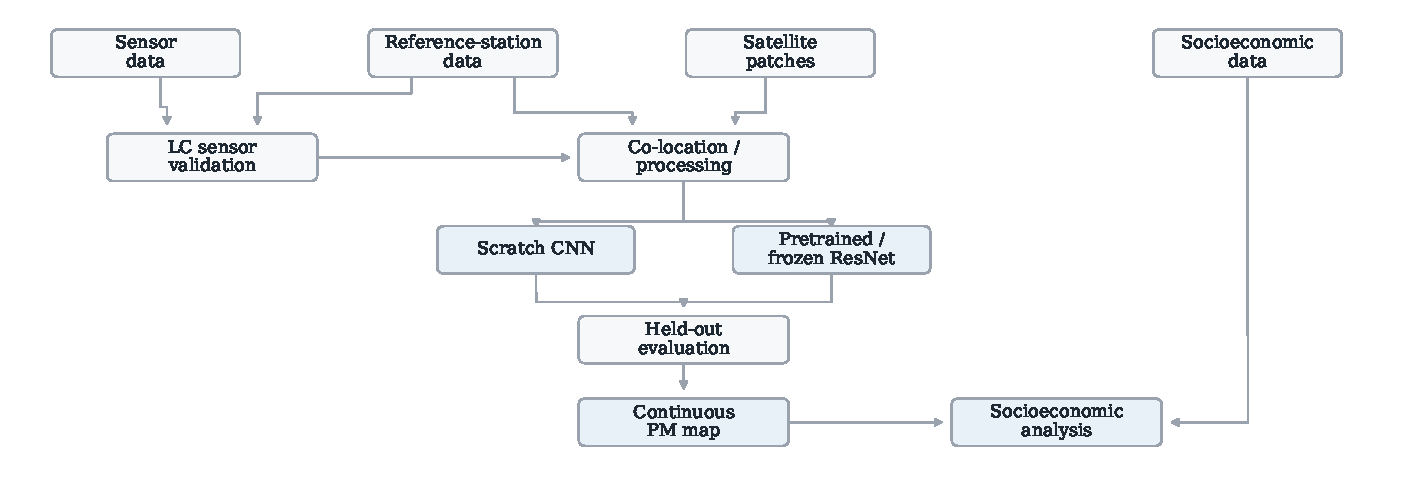
\includegraphics[width=0.9\textwidth]{Figures/generated/pipeline_overview_compact.pdf}
    \caption{Pipeline Overview.}
    \label{fig:pipeline_overview}
\end{figure}

%introduction socio-economic analysis 
%   references to previous pollution impact analyses 

%possible visual with the pipeline, as a nice overview 

The remainder of this report is structured as follows. Section 2 describes the data and processing steps. Section 3 presents the low-cost sensor calibration. Section 4 describes the model architectures. Section 5 presents the predictive results. Section 6 covers the socioeconomic analysis and Section 7 concludes. The code and supporting project files are available at \url{https://github.com/simone-mazzoli/air_pollution}.

\section{Data Collection and Processing}

In this section, we describe the data sources used in this project and the processing steps applied to produce valid, model-ready training data.

We use three main categories of data: particulate matter (PM) measurements, satellite patches including pollution covariates and socioeconomic data. Figure~\ref{fig:pipeline_overview} provides an overview of the different data types used. Unless otherwise specified, the data refer to the year 2024.

%figure with overview of data types 

\subsection{PM Data}

We gather PM measurements that serve as labels for our models to train. Low-cost (LC) sensor measurements are gathered from Sensor.Community \citep{sensorcommunity2026}, while reference stations across Europe (EEA stations) are fetched using the EEA API \citep{eea_aqereporting}. Sensor.Community is a non-profit organization that collects data from private sensors. They supply information for how private actors can install a home sensor and collect the data from sensors connected to their network. They provide access to approximately ten thousand sensors globally. The EEA collects data from local and regional authorities and creates uniform datasets with environmental data across Europe. The Sensor.Community sensors are abundant and cover many areas not extensively covered by the EEA stations, while the latter provide high quality measurements to test the low cost sensors' validity.


%preprocessing decisions 
Annual station means were constructed after applying a joint PM10/PM2.5 completeness filter during preprocessing. Invalid values include missing or negative values and values marked invalid by the stations themselves. The model loader then keeps stations with a valid PM2.5 annual mean and all required satellite and covariate data. The PM values are averaged over the full year to create annual averages for each station. They are log-transformed and standardized based on the training set mean and standard deviation. Outliers above a value of 120 ug/m3 PM10 and 80 ug/m3 PM2.5 are removed.

%resulting distributions 
%   figure distribution of PM measures 
%   facetted distribution of PM across the folds? 

\begin{figure}[ht]
\centering
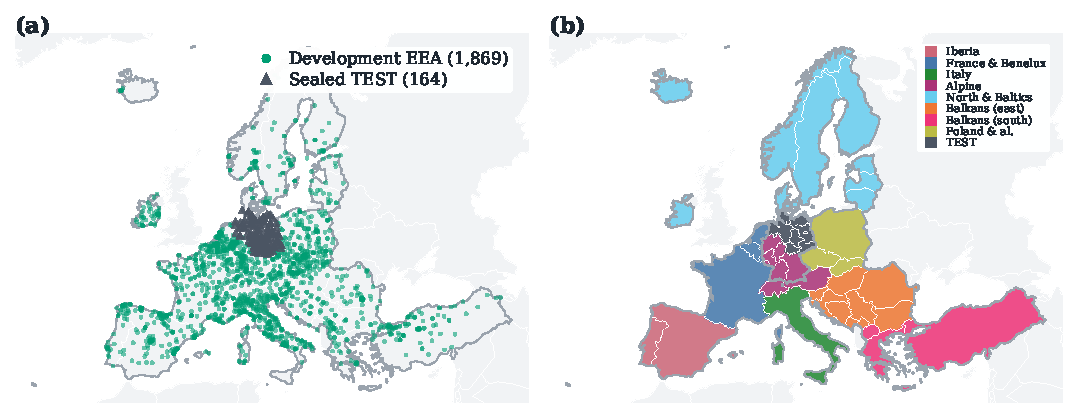
\includegraphics[width=\textwidth]{Figures/generated/coverage_validation_geography.pdf}
\caption{Reference-station coverage and geographic validation design.}
\label{fig:sensor_map}
\label{fig:fold_map}
\end{figure}

Figure~\ref{fig:sensor_map} shows the resulting geographical distribution of EEA reference stations. Station density differs substantially across Europe, which makes random station splits inappropriate for evaluating spatial generalization. We therefore use eight geographically defined development folds and keep a separate northern/eastern German TEST region completely outside model development. The TEST region spans ten German L\"ander and contains 164 reference stations. This is a larger geographic holdout than the single-Land setup originally proposed for the project and provides a more demanding final generalization test.

Figure~\ref{fig:fold_map} shows the folds division. This arrangement is implemented to balance the relative geographical size of each fold and the total number of stations. The 100 km buffer reduces spatial dependence between training and validation stations, but it does not fully remove contextual overlap between all image patches.

\begin{figure}[ht]
    \centering
    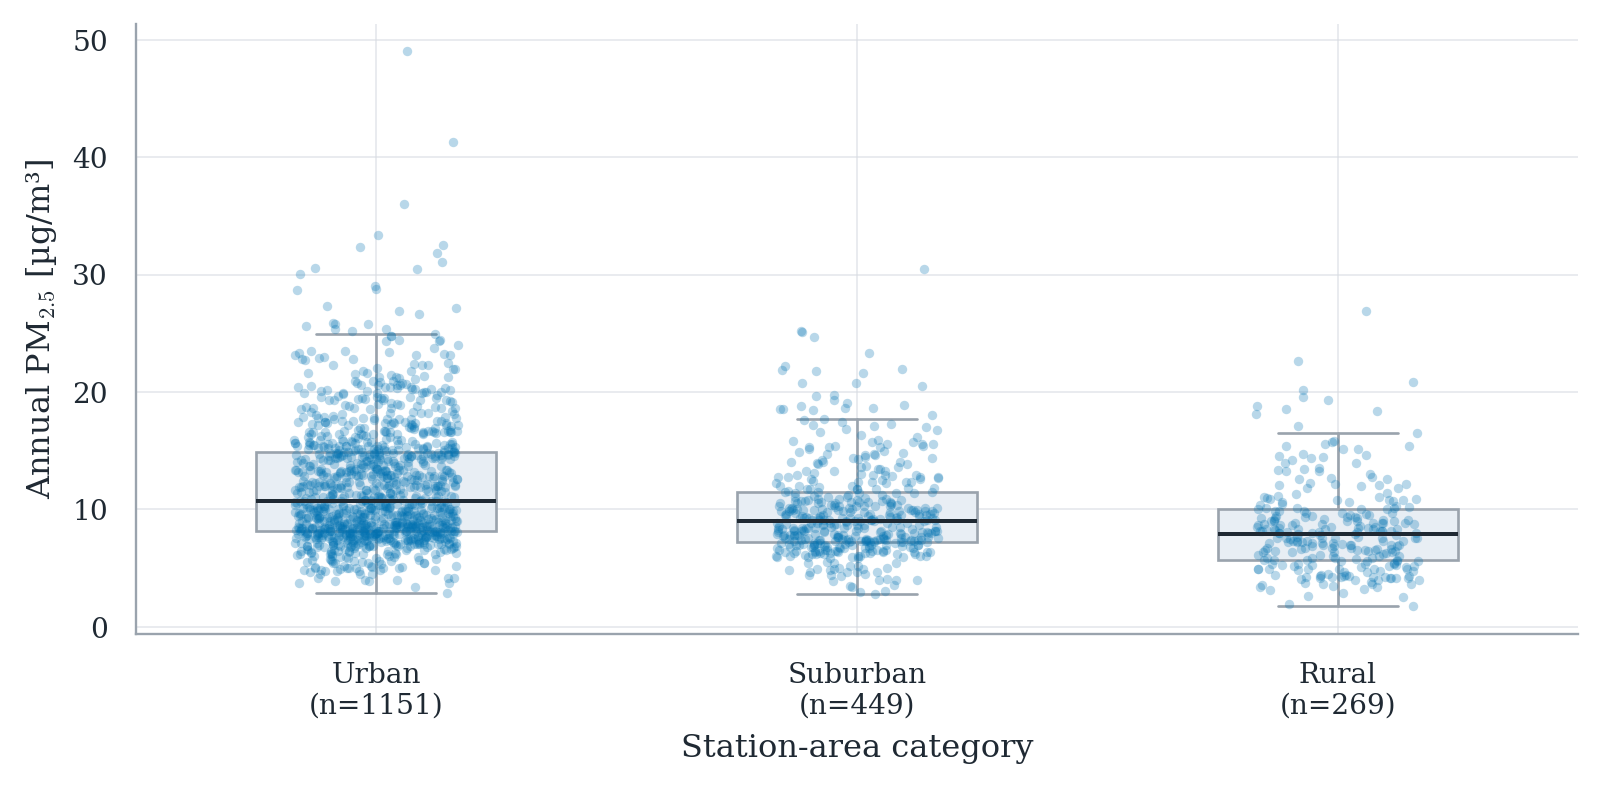
\includegraphics[width=0.82\textwidth]{Figures/generated/urban_rural_pm25_distribution.png}
    \caption{Annual PM2.5 distribution across urban, suburban and rural development stations. The rural group combines rural, rural-nearcity, rural-regional and rural-remote EEA station-area categories.}
    \label{fig:urban_rural_pm25_distribution}
\end{figure}

Using the EEA station-area categories, annual PM2.5 is highest on average at urban development stations, followed by suburban and rural stations. The urban mean is 12.09 \si{\micro\gram\per\cubic\meter} ($n=1151$), the suburban mean is 9.89 ($n=449$) and the combined rural mean is 8.42 ($n=269$). This describes the distribution of station labels and does not explain model performance.




\subsection{Satellite Data}

Satellite patches are fetched through the Google Earth Engine (GEE) API \citep{gorelick2017earthengine}. For each reference station location, we extract Sentinel-2 (S2) multispectral patches \citep{drusch2012sentinel2} at two spatial resolutions: 120 x 120 pixels at a nominal 10 m export spacing for local detail and 60 x 60 pixels at a nominal 200 m export spacing for wider spatial context. The S2 patches are built as cloud-filtered annual median composites. Following the band selection used by the BigEarthNet-pretrained ResNet50, we keep ten of the thirteen total Sentinel-2 bands. We therefore exclude coastal aerosol, water vapor and cirrus. The satellite images are augmented during training by random rotations in increments of 90 degrees.

\begin{figure}[ht]
    \centering
    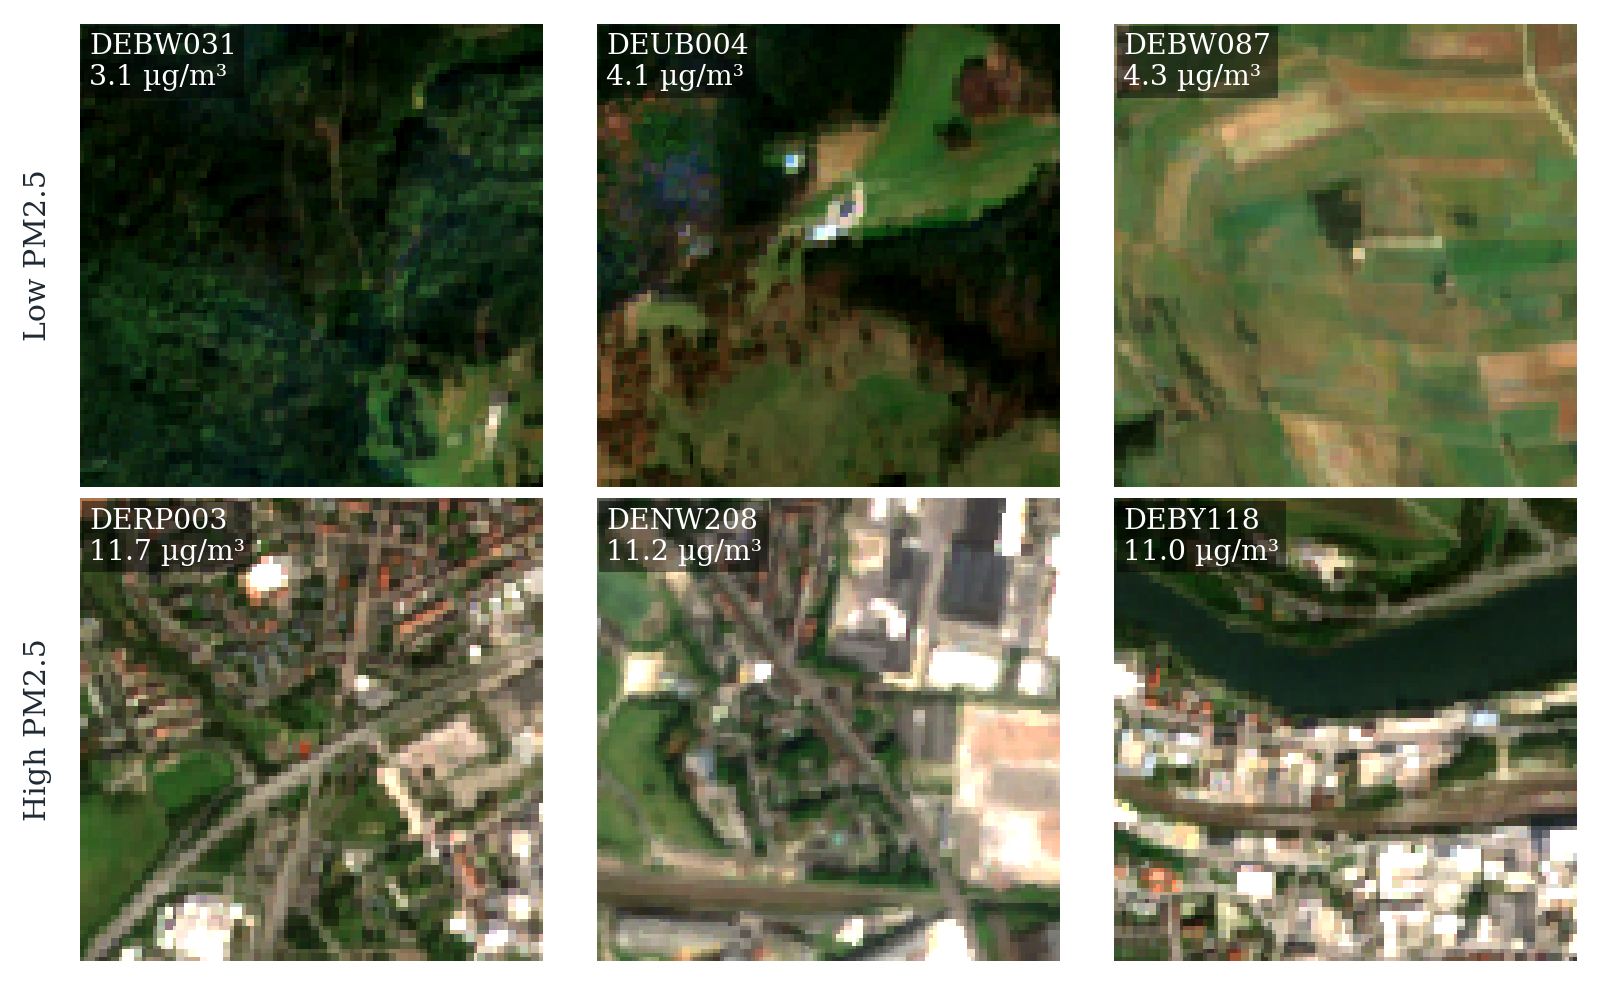
\includegraphics[width=0.78\textwidth]{Figures/generated/high_low_pm25_patch_examples.png}
    \caption{High-resolution Sentinel-2 true-color patch examples for relatively low and relatively high PM2.5 German development stations. All shown stations have at least 330 valid PM2.5 days in 2024.}
    \label{fig:high_low_pm25_patch_examples}
\end{figure}

Figure~\ref{fig:high_low_pm25_patch_examples} shows three relatively low and three relatively high PM2.5 German development stations. The low examples are rural-regional stations, while the high examples are urban stations. The figure is illustrative and should not be read as evidence for what the CNN learned internally. The corresponding low-resolution Sentinel-2 patches are shown in Figure~\ref{fig:high_low_pm25_patch_examples_lowres} in the appendix.



%explanation data source 
%how did we get it 

\subsection{Pollution Covariates}

In addition to S2 imagery, we incorporate four auxiliary covariates through the same GEE pipeline. Sentinel-5P (S5P) atmospheric column data provide tropospheric NO2 and CO measurements using 5 x 5 pixel patches at nominal 7 km export spacing \citep{veefkind2012tropomi}. We also use aerosol index data over a wider 31 x 31 pixel nominal projected footprint. The widest aerosol context is larger than the 100 km buffer, so some contextual overlap can remain even though PM labels are still separated by the validation split. S5P patches are generated as annual mean composites. In addition, we obtain elevation data from the Copernicus GLO-30 digital elevation model (DEM) \citep{esa2021copernicusdem}.

%explanation data source and relevance
%how did we get it 

%potentially a heatmap, how are they related to PM as justification for their inclusion, 

\subsection{Socioeconomic Data}

To examine whether modeled air pollution is spatially associated with
socioeconomic and demographic characteristics, we construct a dataset at the
German Kreis level. The dataset covers all 400 Kreise and combines information
from several official sources. Population, age structure, median age and
population density refer to 2024 and are obtained from Eurostat
\citep{eurostat_pjanaggr3,eurostat_pjanind3,eurostat_d3dens}. Kreis-level
unemployment rates for 2024 are obtained from the German Federal Employment
Agency \citep{ba_arbeitslosenquoten2024}. Disposable household income per capita is taken from the Regional
Accounts of the German States (VGRdL) and refers to 2023 \citep{vgrdl_r2b3_2023}. Finally, indicators
of immigration history, nationality and educational attainment are derived
from the 2022 German Census \citep{zensus2022_demografie,zensus2022_bildung}. Administrative Kreis identifiers and boundaries
are based on official BKG geodata \citep{bkg_vg250_2024}.

Because the most recent available observation year differs across data
sources, we retain the original reference year of each variable. The socioeconomic variables
therefore describe broadly contemporaneous, but not perfectly synchronous
conditions between 2022 and 2024.

For the subsequent analysis, we focus on disposable income, unemployment,
educational attainment, immigration history, population density and age
structure. Immigration history is treated as a demographic characteristic
rather than as an indicator of socioeconomic disadvantage. Population density
is included because urbanicity may be associated with both socioeconomic
characteristics and pollution.

The selected socioeconomic indicators vary strongly across German Kreise.
Population density is especially right-skewed, with a small number of highly
urbanized Kreise having much larger densities than the majority of districts.
The indicators are also related to one another. For example, disposable income
and unemployment are negatively correlated ($r=-0.64$), while immigration
history is positively correlated with both population density ($r=0.72$) and
the share of the population without a vocational qualification ($r=0.79$).
These relationships are important when interpreting associations with
predicted pollution, since spatial differences in one socioeconomic
characteristic may partly reflect differences in another. The distributions
of the selected indicators and their full correlation matrix are shown in
Figures~\ref{fig:socioeconomic_distributions} and
\ref{fig:socioeconomic_correlations} in the appendix.

\section{Calibration of LC PM Sensors}

Before using Sensor.Community measurements as additional labels, we test whether the low-cost SDS011 measurements can be calibrated against nearby German reference stations. Sensor.Community coverage is participation-driven rather than designed to be representative, so regions with fewer participating households can remain undermeasured. Since we do not use these measurements as final model labels, this source of selection does not directly enter the final training labels although the official reference network is also spatially uneven. Humidity can introduce systematic bias in low-cost PM measurements, so annual averaging alone does not guarantee unbiased labels. This is one reason why we also test the weather-aware calibration below. We first compare the raw annual SDS011 measurements with a constant reference-mean baseline and several calibration methods. The baseline predicts the training reference mean for each held-out station. If a calibration method is useful for our purpose, it should improve on this baseline while still preserving meaningful spatial differences between stations.

We test national percentile and range mapping as well as OLS and Huber regression. For the regression approaches, the reference-station concentration is the dependent variable and the nearby low-cost sensor measurement is the main predictor. The annual regression comparison is evaluated with leave-one-Land-out folds over the non-Sachsen-Anhalt development Länder. A related remote calibration approach is discussed by \citet{weissert2023moma}.

\begin{table}[ht]
\centering
\small
\caption{Summary of the main Sensor.Community calibration experiments. Annual values report station-balanced RMSE in \si{\micro\gram\per\cubic\meter}. The HYRAS rows report daily RMSE improvement over the corresponding constant baseline.}
\label{tab:calibration_summary}
\resizebox{\textwidth}{!}{%
\begin{tabular}{lllll}
\hline
 \textbf{Approach}  & \textbf{Pollutant}  &\textbf{Level}  &\textbf{Headline result}  &\textbf{Beat baseline?}  \\
 \hline
constant-mean baseline  &PM10  &annual  &mean RMSE 2.911  &baseline  \\
  &PM2.5  &annual  &mean RMSE 1.836  &baseline  \\
 \hline
 raw SDS011  &PM10  &annual  &mean RMSE 46.310  &no  \\
   &PM2.5  &annual  &mean RMSE 26.959  &no  \\
\hline
 national percentile/range mapping  &PM10  &annual  &mean RMSE 20.860  &no  \\
  &PM2.5  &annual  &mean RMSE 12.559  &no  \\
\hline
 OLS regression adjustment  &PM10  &annual  &mean RMSE 3.098  &no  \\
  &PM2.5  &annual  &mean RMSE 1.919  &no  \\
\hline
 Huber regression adjustment  &PM10  &annual  &mean RMSE 3.157  &no  \\
   &PM2.5  &annual  &mean RMSE 2.169  &no  \\
\hline
 daily weather-aware regression  &PM10  &daily  &RMSE improvement vs constant 2.523  &yes  \\
  &PM2.5  &daily  &RMSE improvement vs constant 2.272  &yes  \\
\hline
 background-station-only sensitivity  &PM10  &annual  &RMSE improvement vs constant -0.395  &no  \\
   &PM2.5  &annual  &RMSE improvement vs constant -0.196  &no  \\
\hline
 clustered-sensor mean  &PM10  &annual  &RMSE 3.108  &no  \\
 clustered-sensor median &PM10  &annual  &RMSE 3.172  &no \\
\hline
\end{tabular}
}
\end{table}

The raw annual SDS011 values have very large errors. OLS and Huber calibration reduce this error considerably, but both remain slightly worse than the constant baseline and strongly compress the spatial variation in the reference values. We therefore also test a daily weather-aware regression using HYRAS temperature and relative humidity data \citep{razafimaharo2020hyras}. The daily model includes raw PM, humidity, temperature and an interaction between raw PM and humidity. It improves RMSE over the daily constant baseline by 2.523 \si{\micro\gram\per\cubic\meter} for PM10 and 2.272 \si{\micro\gram\per\cubic\meter} for PM2.5. The weather-aware daily model shows useful short-term predictive signal.

However, this improvement does not carry over to the annual labels we need for model training. The annual background-station check still performs worse than the constant baseline and combining nearby low-cost sensors does not clearly improve the estimates either. We therefore do not conclude that low-cost sensors are generally unusable. Instead, the tested Sensor.Community calibration approaches do not provide annual labels that are accurate and spatially informative enough for the final model. Sensor.Community is therefore excluded from model training and the development dataset is expanded to EEA reference stations across Europe.

\section{Models}
We trained two model families. Firstly, we trained a CNN constructed from scratch. Secondly, we evaluated ResNet-50 based variants using a backbone pretrained on BigEarthNet v2 imagery \citep{he2015deepresiduallearningimage,clasen2025refinedbigearthnet}. This lets us test whether using a backbone pretrained on satellite imagery improves PM2.5 prediction in our multimodal setup.

\subsection{CNN created from scratch}
\label{sec:cnn_scratch}


% # CNN architecture
\begin{table}[ht]
\centering
\caption{Architecture of the selected scratch multi-input CNN (\texttt{cnn\_deep\_wide}). Each image modality is processed by a separate CNN branch before the resulting feature representations are normalized and combined with scalar context.}
\label{tab:cnn_deep_wide_architecture}
\resizebox{\textwidth}{!}{%
\begin{tabular}{llll}
\hline
\textbf{Branch} & \textbf{Block} & \textbf{Channels} & \textbf{Operations} \\
\hline

High-resolution &
Block 1 & 48 &
3 $\times$ [Conv $3\times3$ $\rightarrow$ BatchNorm $\rightarrow$ ReLU] $\rightarrow$ MaxPool \\
&
Block 2 & 96 &
3 $\times$ [Conv $3\times3$ $\rightarrow$ BatchNorm $\rightarrow$ ReLU] $\rightarrow$ MaxPool \\
&
Block 3 & 192 &
3 $\times$ [Conv $3\times3$ $\rightarrow$ BatchNorm $\rightarrow$ ReLU] $\rightarrow$ MaxPool \\
&
Block 4 & 384 &
3 $\times$ [Conv $3\times3$ $\rightarrow$ BatchNorm $\rightarrow$ ReLU] $\rightarrow$ MaxPool \\
&
Output & 384 &
Global Average Pooling \\
\hline

Low-resolution &
Block 1 & 32 &
Conv $3\times3$ $\rightarrow$ BatchNorm $\rightarrow$ ReLU $\rightarrow$ MaxPool \\
&
Block 2 & 128 &
Conv $3\times3$ $\rightarrow$ BatchNorm $\rightarrow$ ReLU \\
\hline

Sentinel-5P (NO2, CO) &
Block 1 & 32 &
Conv $3\times3$ $\rightarrow$ BatchNorm $\rightarrow$ ReLU \\
&
Block 2 & 32 &
Conv $3\times3$ $\rightarrow$ BatchNorm $\rightarrow$ ReLU \\
&
Output & 32 &
Global Average Pooling \\
\hline

Wide-Aerosol &
Block 1 & 32 &
Conv $3\times3$ (stride 2) $\rightarrow$ BatchNorm $\rightarrow$ ReLU \\
&
Block 2 & 32 &
Conv $3\times3$ (stride 2) $\rightarrow$ BatchNorm $\rightarrow$ ReLU \\
&
Output & 32 &
Global Average Pooling \\
\hline

DEM &
Block 1 & 32 &
Conv $3\times3$ $\rightarrow$ BatchNorm $\rightarrow$ ReLU $\rightarrow$ MaxPool \\
&
Block 2 & 32 &
Conv $3\times3$ $\rightarrow$ BatchNorm $\rightarrow$ ReLU \\
&
Output & 32 &
Global Average Pooling \\
\hline

Fusion &
Normalization & -- &
Normalize outputs of all five CNN branches \\
&
Scalar context & -- &
NO2/CO patch means, aerosol center-pixel value, elevation \\
\hline

\end{tabular}
}
\end{table}


The CNN created from scratch combines separate branches for the high-resolution Sentinel-2 patch, the low-resolution Sentinel-2 patch, Sentinel-5P inputs, wide aerosol context and DEM elevation. The high-resolution branch has four convolutional blocks with increasing channel size. The smaller input branches use shallower CNNs. Their outputs are normalized before they are combined with scalar context values in the regression head. These scalar values are the NO2 patch mean, the CO patch mean, the center-pixel value of the wide aerosol patch and station elevation.


\begin{table}[ht]
\centering
\caption{Hyperparameters for the scratch CNN (\texttt{cnn\_deep\_wide}).}
\label{tab:cnn_deep_wide_hparams}
\begin{tabular}{ll}
\hline
\textbf{Hyperparameter} & \textbf{Value} \\
\hline
High-resolution channels & 48 $\rightarrow$ 96 $\rightarrow$ 192 $\rightarrow$ 384 \\
Conv layers per block & 3 \\
Learning rate & $3\times10^{-4}$ \\
Weight decay & $1\times10^{-7}$ \\
Dropout & 0.5 \\
Batch size & 128 \\
Projection dim & 64 \\
Low-res CNN channels & 32 $\rightarrow$ 128 \\
Sentinel-5P CNN hidden width & 32 \\
Wide-aerosol feature dim & 32 \\
DEM feature dim & 32 \\
Regression head hidden width & 64 \\
Spatial buffer & 100 km \\
TTA & enabled (8 views) \\
Max epochs / patience & 500 / 25 \\
\hline
\end{tabular}
\end{table}




\subsection{ResNet-50 Based Model}

The ResNet-50 variant replaces the scratch high-resolution encoder with a ResNet-50 pretrained on BigEarthNet v2, also referred to as reBEN \citep{clasen2025refinedbigearthnet}. The pretrained model uses the same ten Sentinel-2 bands as the high-resolution scratch branch. Only the high-resolution Sentinel-2 patch passes through this backbone. Every other data modality uses the same scratch CNN branches described in Subsection~\ref{sec:cnn_scratch}. The comparison therefore asks whether the evaluated pretrained representation improves annual station-level PM2.5 regression in our multimodal setup.
We experiment with several hyperparameter configurations, especially varying the freezing or unfreezing of the backbone layers, the learning rate and the dropout rate. Table~\ref{tab:resnet_frozen_architecture} reports the architecture of the frozen ResNet variant used for the main comparison, which only differs from \texttt{cnn\_deep\_wide} in the High-resolution branch. It uses a frozen backbone, a head learning rate of $1\times10^{-5}$ and a dropout rate of 0.8; all other hyperparameters are identical to \texttt{cnn\_deep\_wide} (Table~\ref{tab:cnn_deep_wide_hparams}). A backbone-trainable diagnostic was evaluated only on the Iberia fold and gave a similar result to the frozen variant.



\begin{table}[ht]
\centering
\caption{Architecture of the frozen-backbone multi-input model. The high-resolution branch uses a BigEarthNet-pretrained ResNet50 with 10-channel input as a fixed feature extractor. Only the projection after the backbone is trainable. The low-resolution, Sentinel-5P, wide-aerosol, DEM and fusion branches are identical to \texttt{cnn\_deep\_wide} (Table~\ref{tab:cnn_deep_wide_architecture}).}
\label{tab:resnet_frozen_architecture}
\begin{tabular}{llll}
\hline
\textbf{Branch} & \textbf{Block} & \textbf{Channels} & \textbf{Operations} \\
\hline
High-resolution &
Stem & 64 &
Conv $7\times7$ $\rightarrow$ BatchNorm (frozen) $\rightarrow$ ReLU $\rightarrow$ MaxPool \\
&
Layer 1 & 256 &
3 $\times$ Bottleneck [Conv $1\times1$ $\rightarrow$ Conv $3\times3$ $\rightarrow$ Conv $1\times1$], frozen \\
&
Layer 2 & 512 &
4 $\times$ Bottleneck, frozen \\
&
Layer 3 & 1024 &
6 $\times$ Bottleneck, frozen \\
&
Layer 4 & 2048 &
3 $\times$ Bottleneck, frozen \\
&
Output &
64 &
Global Average Pooling $\rightarrow$ Linear projection (trainable) \\
\hline
\end{tabular}
\end{table}






\section{Results}
\label{sec:results}

\subsection{Training}

Both models are trained under identical leave-one-fold-out cross-validation: eight geographically defined development folds. Each fold takes a turn as the validation fold, with the model trained on the remaining seven. Training stations within 100 km of any validation station are removed from that fold's training set to reduce spatial dependence between neighbouring, highly correlated locations. The northern/eastern German TEST region is never used at this stage. It is sealed until the final evaluation in Section~\ref{sec:results}. Both models are trained with early stopping, using a patience of 25 epochs and a maximum of 500 epochs.

Best-epoch selection varies substantially across folds. For the scratch CNN, the best epoch ranges from 1 to 71. For the frozen ResNet-50 variant, it ranges from 1 to 424. These large differences suggest that some geographic folds are much harder than others and that the per-fold results should be interpreted together with the pooled result. The corresponding training curves for the scratch CNN and frozen ResNet are shown in Figures~\ref{fig:learning_curves_cnn} and \ref{fig:learning_curves_resnet} in the appendix.


\paragraph{Data size ablation}
We repeat the geographic cross-validation using 25\%, 50\% and 100\% of the available development training data. The 100 km buffer is applied before subsampling and the reduced subsets are sampled within the geographic training folds. The 25\% and 50\% results average three subset-selection seeds, while the 100\% point is the single full-data CV run. Figure~\ref{fig:data_size_rmse_learning_curve} shows that the scratch CNN remains fairly stable across the tested fractions, with RMSE values of 3.846, 3.917 and 3.823. The scratch CNN changes only slightly across these dataset sizes and the differences are not monotonic, so we do not take the 25\% or 50\% results as evidence that using less data is better. The frozen ResNet remains worse at every tested fraction. Overall, reducing the training data does not reveal a transfer-learning advantage for the evaluated ResNet setup.

\begin{figure}
     \centering
     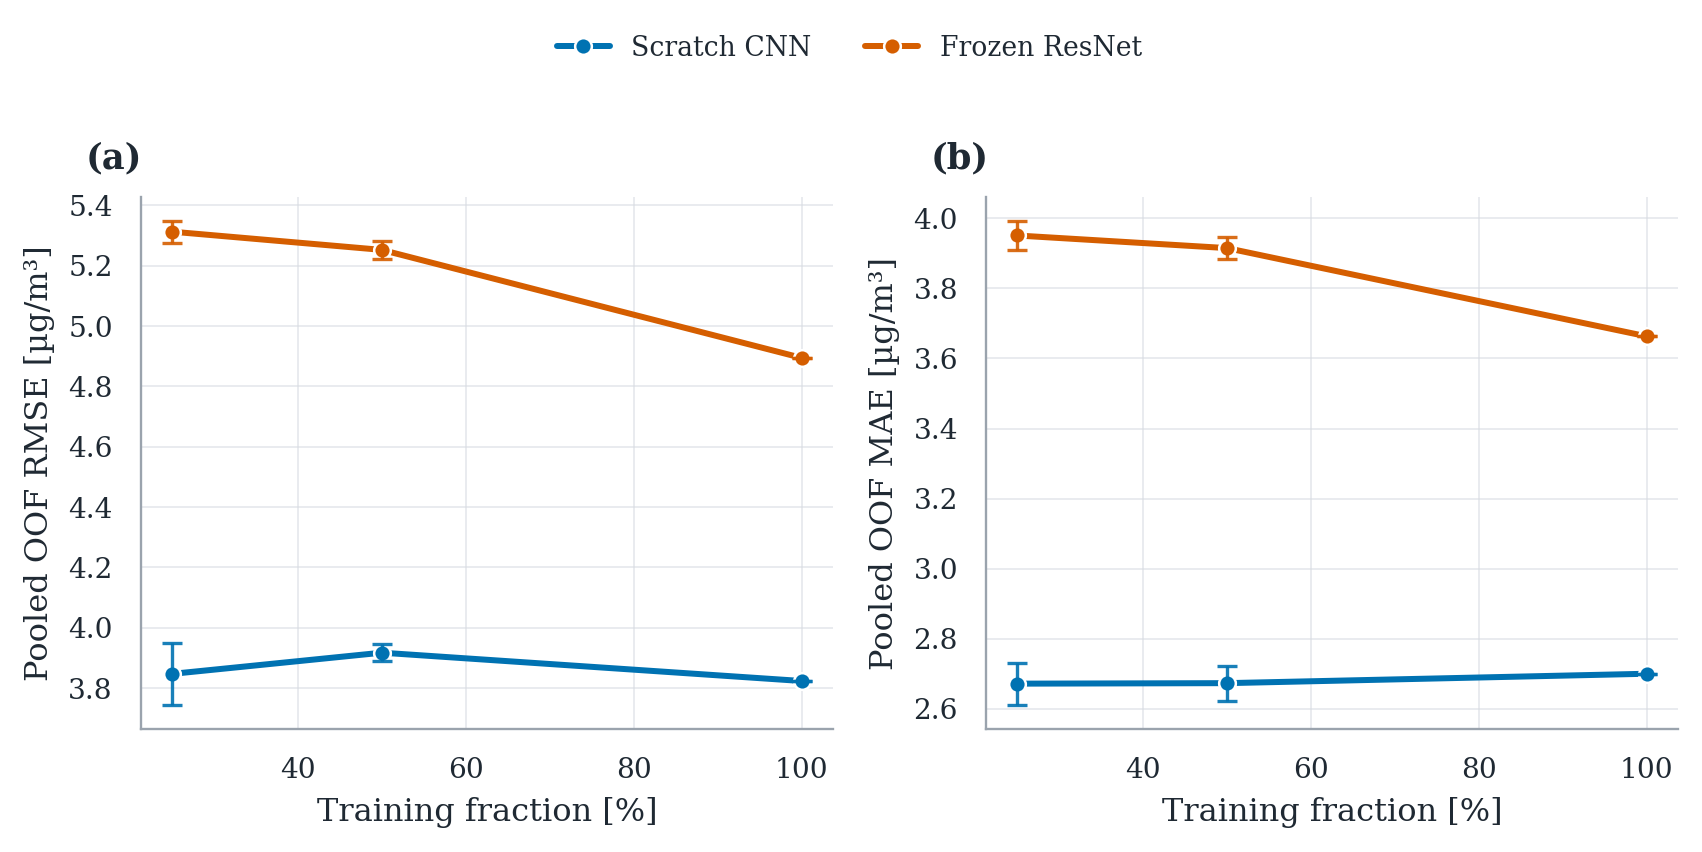
\includegraphics[width=0.92\textwidth]{Figures/generated/data_size_ablation_summary.png}
     \caption{Pooled geographic cross-validation RMSE and MAE for the scratch CNN and frozen ResNet-50 using 25\%, 50\% and 100\% of the development training data.}
     \label{fig:data_size_rmse_learning_curve}
     \label{fig:data_size_mae_learning_curve}
\end{figure}

%explanation why this is necessary 
%results from the datasize ablation

\subsection{Evaluation}

\begin{table}[ht]
\centering
\caption{Cross-validation results, pooled out-of-fold ($n=1869$), PM2.5.}
\label{tab:main_model_comparison}
\begin{tabular}{lccc}
\hline
\textbf{Model} & \textbf{RMSE} & \textbf{MAE} & \textbf{R}$^2$ \\
\hline
Scratch CNN (\texttt{cnn\_deep\_wide}) & 3.823 & 2.700 & 0.417 \\
Frozen ResNet50 backbone & 4.895 & 3.663 & 0.045 \\
\hline
\end{tabular}
\end{table}

The scratch CNN outperforms the frozen-backbone ResNet across all three pooled cross-validation metrics (Table~\ref{tab:main_model_comparison}), with a substantially lower RMSE (3.823 vs.\ 4.895) and higher R\textsuperscript{2} (0.417 vs.\ 0.045). The positive pooled R\textsuperscript{2} should be interpreted together with the individual folds. Five of the eight geographic folds have negative R\textsuperscript{2}, which indicates that broad between-region differences are captured more reliably than within-region variation in several unseen regions. The complete per-fold results for both model families are reported in Tables~\ref{tab:cnn_deep_wide_folds} and \ref{tab:resnet_frozen_folds} in the appendix.

We selected \texttt{cnn\_deep\_wide} before opening the sealed TEST set. In the original pre-TEST scratch comparison, \texttt{cnn\_deep\_wide} had a pooled CV RMSE of 3.746 and the compact CNN had 3.797. The eight original best epochs were 16, 22, 25, 25, 20, 42, 34 and 22, giving a median of 23.5 and a final training length of 24 epochs. Before final fitting, the 100 km buffer around the TEST region removed 74 of the 1,869 development stations, leaving 1,795 stations for the 24-epoch final fit. A later reproducibility rerun put the two scratch models very close together, with RMSE 3.823 for \texttt{cnn\_deep\_wide} and 3.809 for the compact CNN. We keep the earlier model choice because the architecture and 24-epoch final training choice had already been fixed before TEST evaluation. The evaluated BigEarthNet-pretrained ResNet configurations did not outperform the scratch CNN. The backbone-trainable ResNet diagnostic was only evaluated on the Iberia fold, where it was similar to the frozen variant.

\begin{table}[ht]
\centering
\caption{Final evaluation on the sealed TEST region (northern/eastern Germany, PM2.5, \texttt{cnn\_deep\_wide}, $n=164$).}
\label{tab:test_summary}
\begin{tabular}{lc}
\hline
\textbf{Metric} & \textbf{Value} \\
\hline
MAE & 1.894 \\
RMSE & 2.375 \\
R$^2$ (vs. TEST-set mean) & -1.750 \\
Bias (mean prediction $-$ mean observation) & +1.748 \\
Fraction of stations overpredicted & 87.2\% \\
Training-mean baseline RMSE & 2.782 \\
RMSE improvement over training-mean baseline & 14.6\% \\
\hline
\end{tabular}
\end{table}

Table~\ref{tab:test_summary} reports the model's performance on the 164 sealed TEST stations, never seen during development. The negative R\textsuperscript{2} indicates that the model explains within-TEST variation poorly relative to predicting the TEST set's own mean. That mean is only knowable after observing the held-out labels, so we also compare against a deployable training-mean baseline. Relative to this baseline the model reduces RMSE by 14.6\%. Both results are relevant. The model improves on the training-only constant prediction while still showing weak within-region explanatory power. It also has a clear systematic bias, with 87.2\% of TEST stations overpredicted by 1.75 \si{\micro\gram\per\cubic\meter} on average.

State-level TEST summaries vary considerably and several states contain only a small number of reference stations. Berlin is the only state with positive R\textsuperscript{2}, but the subgroup results are too small and unstable to support broader claims about urban or rural reliability. The state-level results are reported as a diagnostic in Table~\ref{tab:test_by_state} in the appendix.

\subsection{Implementation of Dense Grid Map}

We apply the selected scratch model across the northern/eastern German region on a regular grid with approximately 10 km spacing, producing 1,728 usable point predictions. To turn these points into the continuous map shown in the figure, we construct a Delaunay triangulation and interpolate between the three prediction points at each triangle. The continuous-looking surface in Figure~\ref{fig:continuous_grid_map} is therefore a visualization of the grid predictions rather than a separate model prediction at every displayed pixel.

\begin{figure}[ht]
    \centering
    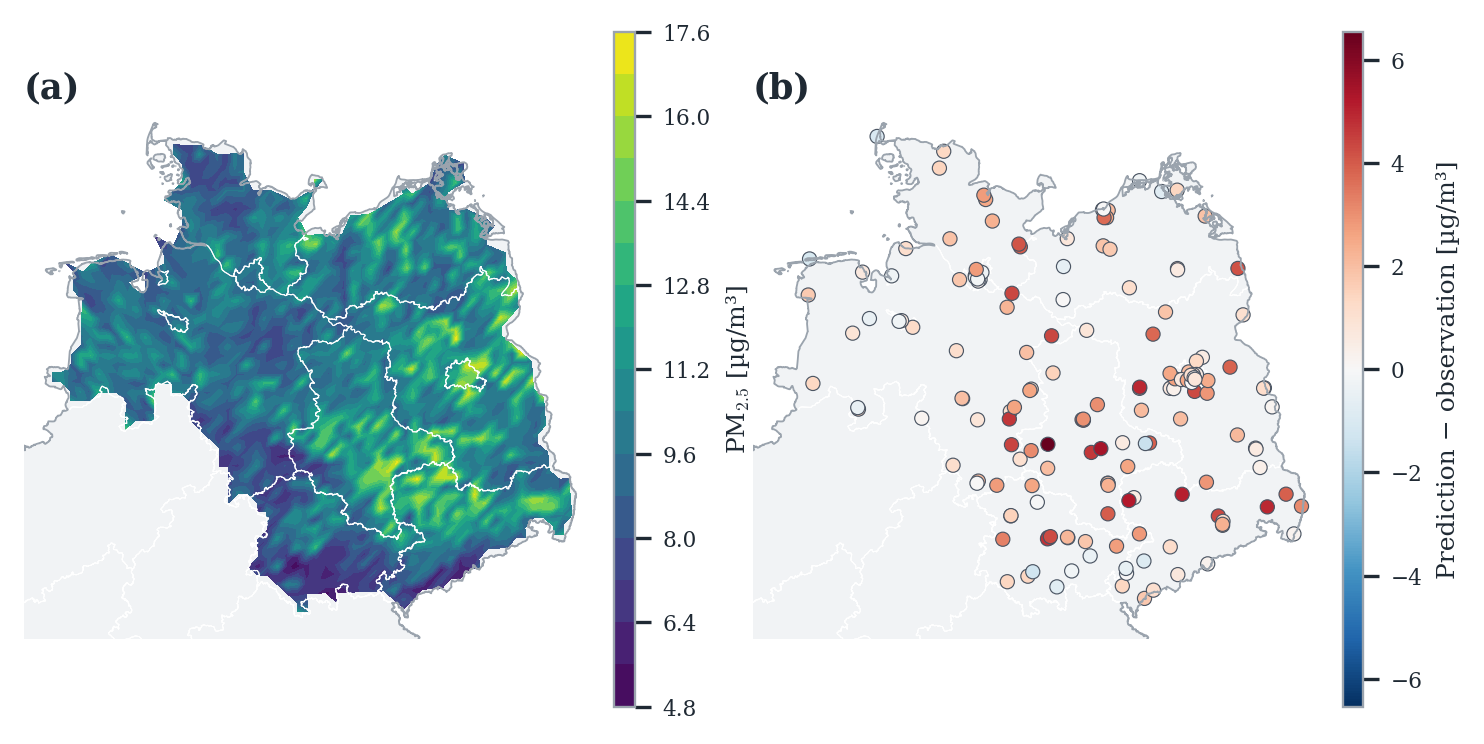
\includegraphics[width=\textwidth]{Figures/generated/dense_prediction_residual_maps.png}
    \caption{Interpolated surface from regular-grid PM2.5 model predictions across the TEST region and residuals at the 164 reference stations. The continuous surface is created by interpolation between model prediction points.}
    \label{fig:continuous_grid_map}
    \label{fig:test_residual_map}
\end{figure}

Across the 1,728 grid points, predicted PM2.5 ranges from approximately 5.02 to 17.13 \si{\micro\gram\per\cubic\meter}. The map shows several areas with relatively high predicted values, including around Berlin and Leipzig. However, the TEST results also show systematic overprediction and weak prediction of within-region variation. We therefore treat the map as an exploratory spatial prediction rather than a replacement for monitoring data or a direct ranking of intervention priorities.

\section{Socioeconomic Analysis}

\subsection{Aggregation of predicted PM2.5 to Kreis level}

The dense-grid predictions described in Section~\ref{sec:results} are produced
at regularly spaced locations rather than directly at administrative units.
To combine these predictions with the socioeconomic data, each grid point is
therefore assigned to the Kreis polygon containing its center coordinates.
Predicted PM2.5 is then averaged across all grid points located within each
Kreis.

Of 1,728 usable grid predictions, 1,719 could be assigned to a Kreis. This
results in Kreis-level modeled pollution estimates for 134 Kreise within the
northern/eastern German prediction domain. The number of contributing grid
points varies with Kreis size, ranging from 1 to 54, with a median of 12 grid
points per Kreis.

Our main pollution measure is the arithmetic mean of the predicted PM2.5
values within each Kreis. It should therefore be interpreted as an
area based estimate of mean modeled ambient pollution. It is not weighted by
population and should not be read as individual exposure. Constructing such a
measure would require information on the within-Kreis spatial distribution of
the population.

Across the 134 covered Kreise, mean predicted PM2.5 ranges from approximately
6.02 to 13.12~\si{\micro\gram\per\cubic\meter}, with an overall Kreis mean of
9.88~\si{\micro\gram\per\cubic\meter}.

\subsection{Association with socioeconomic characteristics}

The modeled PM2.5 values and socioeconomic indicators both vary across space.
The corresponding spatial maps are shown in Figure~\ref{fig:socioeconomic_maps} in the appendix.
However, the spatial patterns do not indicate a single, consistent
socioeconomic gradient in modeled pollution. Areas of higher predicted PM2.5
overlap with some relatively dense and urbanized Kreise, but similar pollution
levels also occur across Kreise with different income, unemployment, education
and demographic profiles. 

Table~\ref{tab:pm25_socioeconomic_correlations} reports exploratory area-level
associations with modeled PM2.5, measured as descriptive Pearson correlations
between mean predicted PM2.5 and the selected Kreis-level indicators. The associations are generally weak. The strongest positive
association is observed for unemployment ($r=0.225$), followed by university
degree share ($r=0.198$) and log population density ($r=0.171$). Disposable
income is weakly negatively associated with predicted PM2.5 ($r=-0.145$).
Immigration history shows essentially no linear relationship with predicted
PM2.5 ($r=-0.022$).

\begin{table}[ht]
\centering
\caption{Pearson correlations between Kreis-level mean predicted PM2.5 and
selected socioeconomic and demographic indicators. Correlations are
descriptive and do not imply causal relationships.}
\label{tab:pm25_socioeconomic_correlations}
\begin{tabular}{lcc}
\toprule
\textbf{Indicator} & \textbf{$n$} & \textbf{Pearson $r$} \\
\midrule
Disposable income per capita      & 132 & -0.145 \\
Unemployment rate                 & 134 &  0.225 \\
No vocational qualification       & 134 & -0.153 \\
University degree                 & 134 &  0.198 \\
Immigration history               & 134 & -0.022 \\
Log population density            & 134 &  0.171 \\
Population aged 65+               & 134 & -0.120 \\
\bottomrule
\end{tabular}
\end{table}

Overall, these results provide little evidence for a strong or uniform
socioeconomic gradient in modeled PM2.5 across the study region. The weak
negative association with disposable income and weak positive association
with unemployment are consistent with somewhat higher modeled pollution in
more economically disadvantaged Kreise, but their magnitude is small.
Moreover, other indicators do not follow the same pattern: the share without
a vocational qualification is weakly negatively associated with predicted
PM2.5, while university-degree share is weakly positively associated with it.
The near-zero association with immigration history further illustrates that
the observed spatial patterns cannot be summarized by a single dimension of
social disadvantage.

These results should also be interpreted in light of the limitations of the
pollution estimates themselves. The socioeconomic analysis is based on model
predictions rather than direct measurements and Section~\ref{sec:results}
shows systematic overprediction and heterogeneous predictive performance in
the held-out German region. In addition, the Kreis-level PM2.5 measure is an
unweighted spatial average and does not account for where people live within
each Kreis. Consequently, the analysis should be understood as an exploratory
assessment of spatial associations between modeled ambient pollution and
Kreis-level socioeconomic characteristics, rather than as evidence of causal
environmental inequality or individual exposure differences.

\section{Conclusion}

In this project, we build a model that predicts PM2.5 pollution from publicly available satellite and contextual data. The tested Sensor.Community calibration approaches did not make the measurements reliable enough to replace official reference measurements as annual model labels. We therefore train the final models on EEA reference stations. The selected scratch CNN performs better than the evaluated BigEarthNet-pretrained ResNet configurations in pooled cross-validation and improves on a training-mean baseline in the sealed northern/eastern German TEST region. At the same time, the TEST results show systematic overprediction and weak within-region explanatory power. The socioeconomic analysis should therefore be read as an exploratory area-level comparison with modeled PM2.5 rather than as evidence of causal environmental inequality.

There are several limitations to our project. First, the original preprocessing used a joint PM10/PM2.5 completeness rule, so some PM2.5 stations fall below a literal 90\% PM2.5 completeness threshold. When we restrict the saved predictions to stations meeting the stricter criterion, pooled CV RMSE changes by about 1.7\% and TEST RMSE by less than 1\%. However, this is only a sensitivity check on the existing predictions. It is not a full retraining of the models. The EPSG:3857 export gives nominal rather than exact physical footprint scales, so true ground distances vary with latitude across the Europe-wide training region. The 100 km buffer reduces spatial dependence but does not fully remove contextual overlap. Five of eight geographic CV folds have negative R\textsuperscript{2}. The ResNet comparison also does not isolate pretraining from every architecture and optimization difference. Finally, the dense map inherits the final model's geographic prediction error and the Kreis averages are modeled area-level pollution rather than population-weighted personal exposure.

Future work could test additional meteorological covariates and other pretrained remote-sensing backbones and could quantify predictive uncertainty more directly.

\bibliography{references}
\clearpage
\section*{Appendix}
\appendix

\section{Additional Graphs and Images}

\begin{figure}[ht]
    \centering
    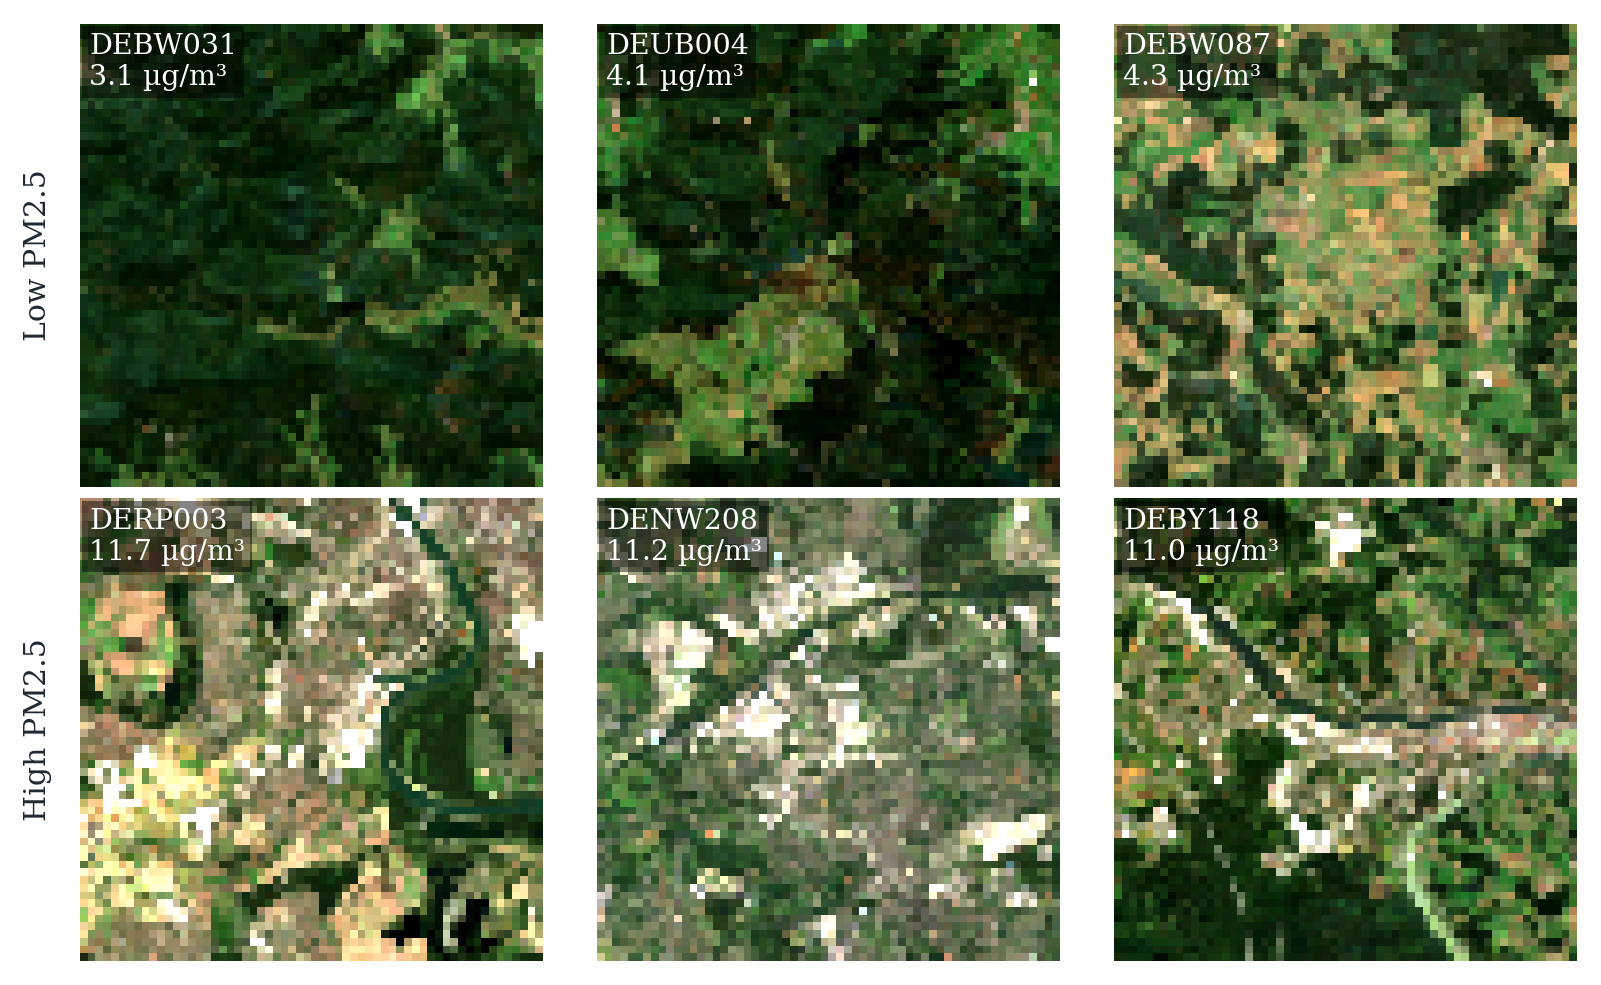
\includegraphics[width=0.8\textwidth]{Figures/generated/high_low_pm25_patch_examples_lowres.png}
    \caption{Low-resolution Sentinel-2 patch examples for the same German stations shown in the main text.}
    \label{fig:high_low_pm25_patch_examples_lowres}
\end{figure}

\begin{figure}[ht]
    \centering
    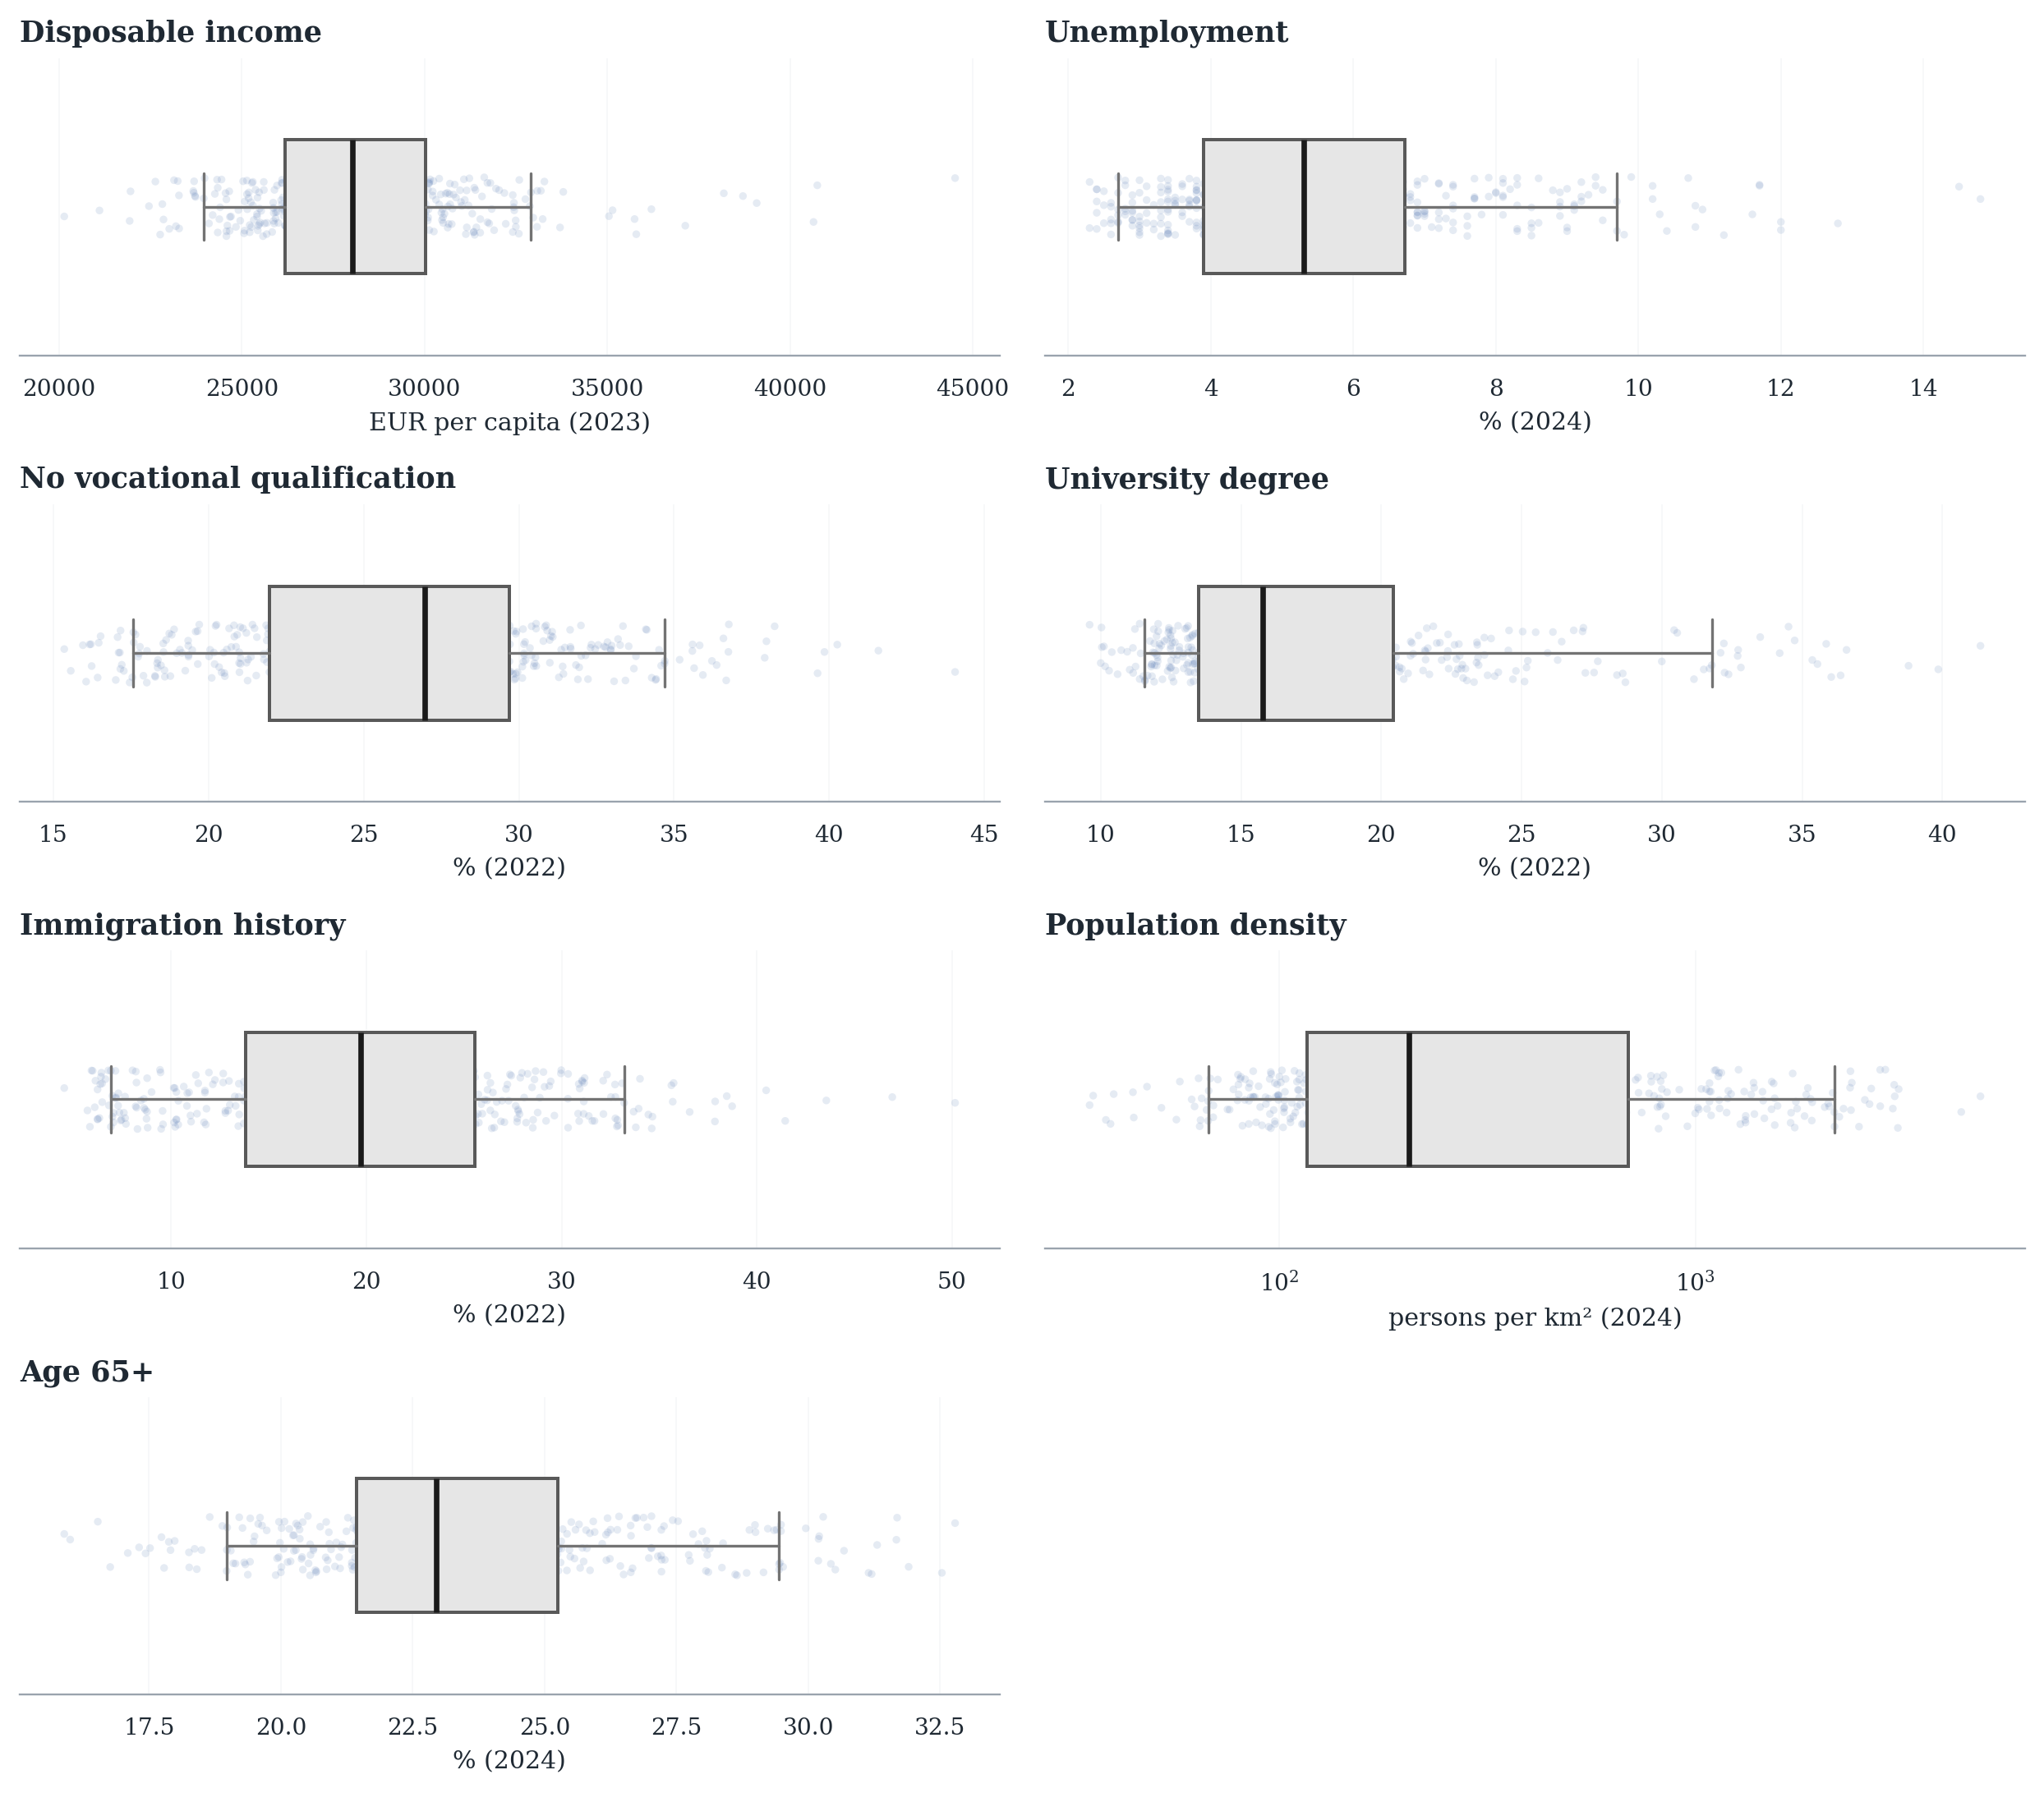
\includegraphics[width=0.75\textwidth]
    {Figures/generated/socioeconomic_indicator_boxplots.png}
    \caption{Distribution of selected socioeconomic and demographic indicators across German Kreise.}
    \label{fig:socioeconomic_distributions}
\end{figure}

\begin{figure}[ht]
    \centering
    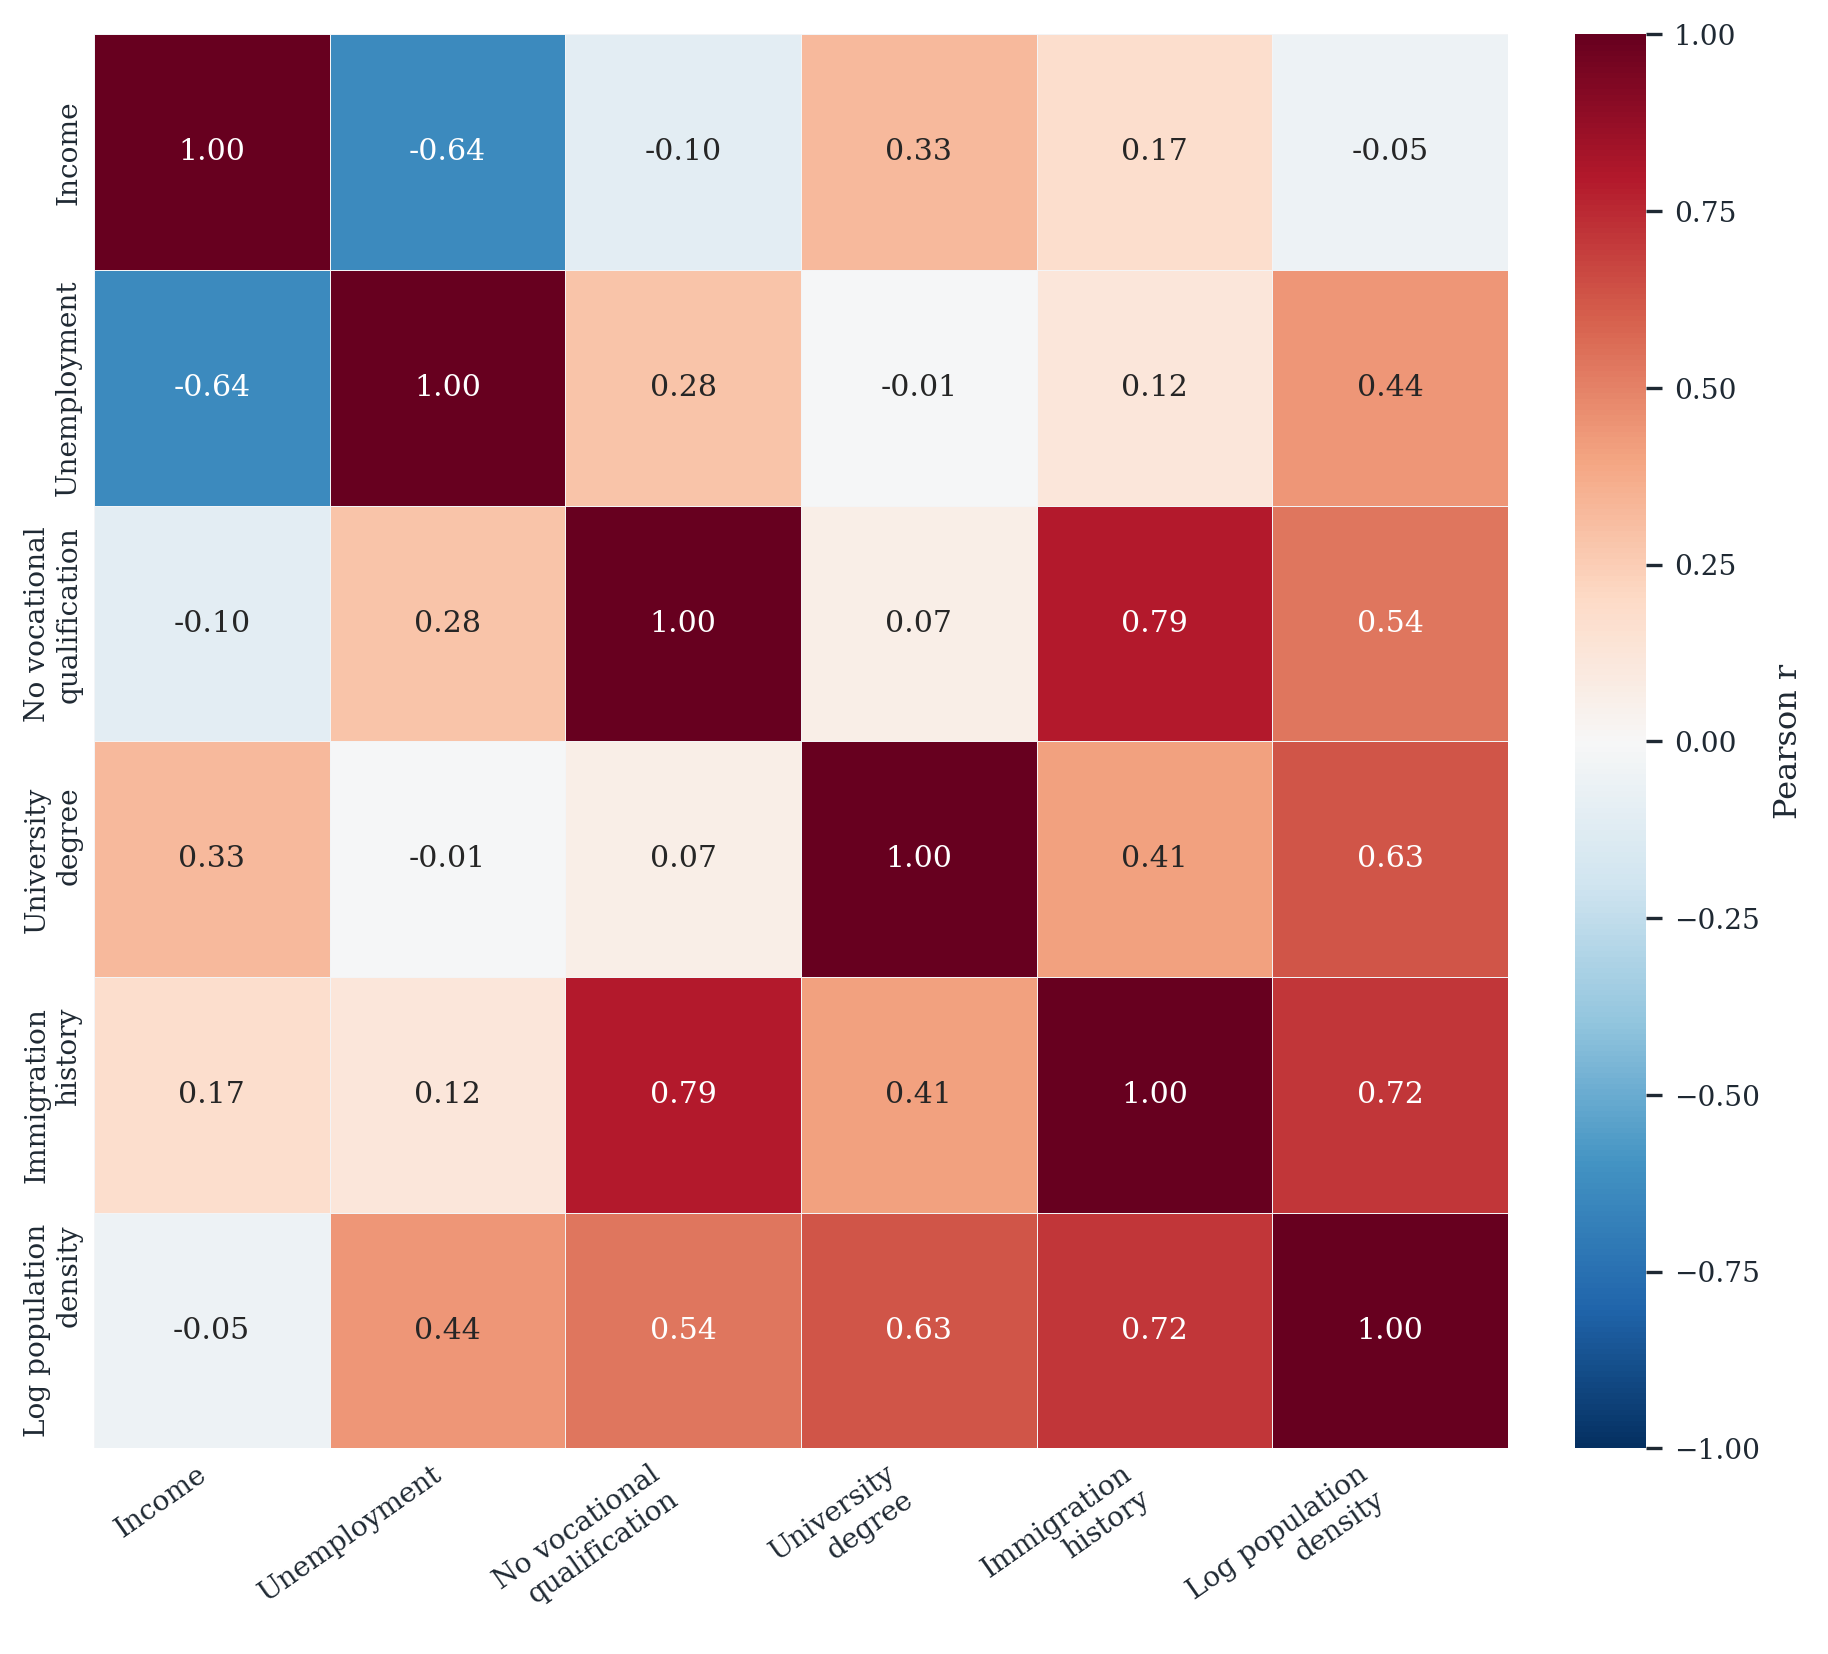
\includegraphics[width=0.65\textwidth]
    {Figures/generated/socioeconomic_correlation_matrix.png}
    \caption{Pearson correlations among selected socioeconomic indicators across German Kreise.}
    \label{fig:socioeconomic_correlations}
\end{figure}

\begin{figure}[ht]
    \centering
    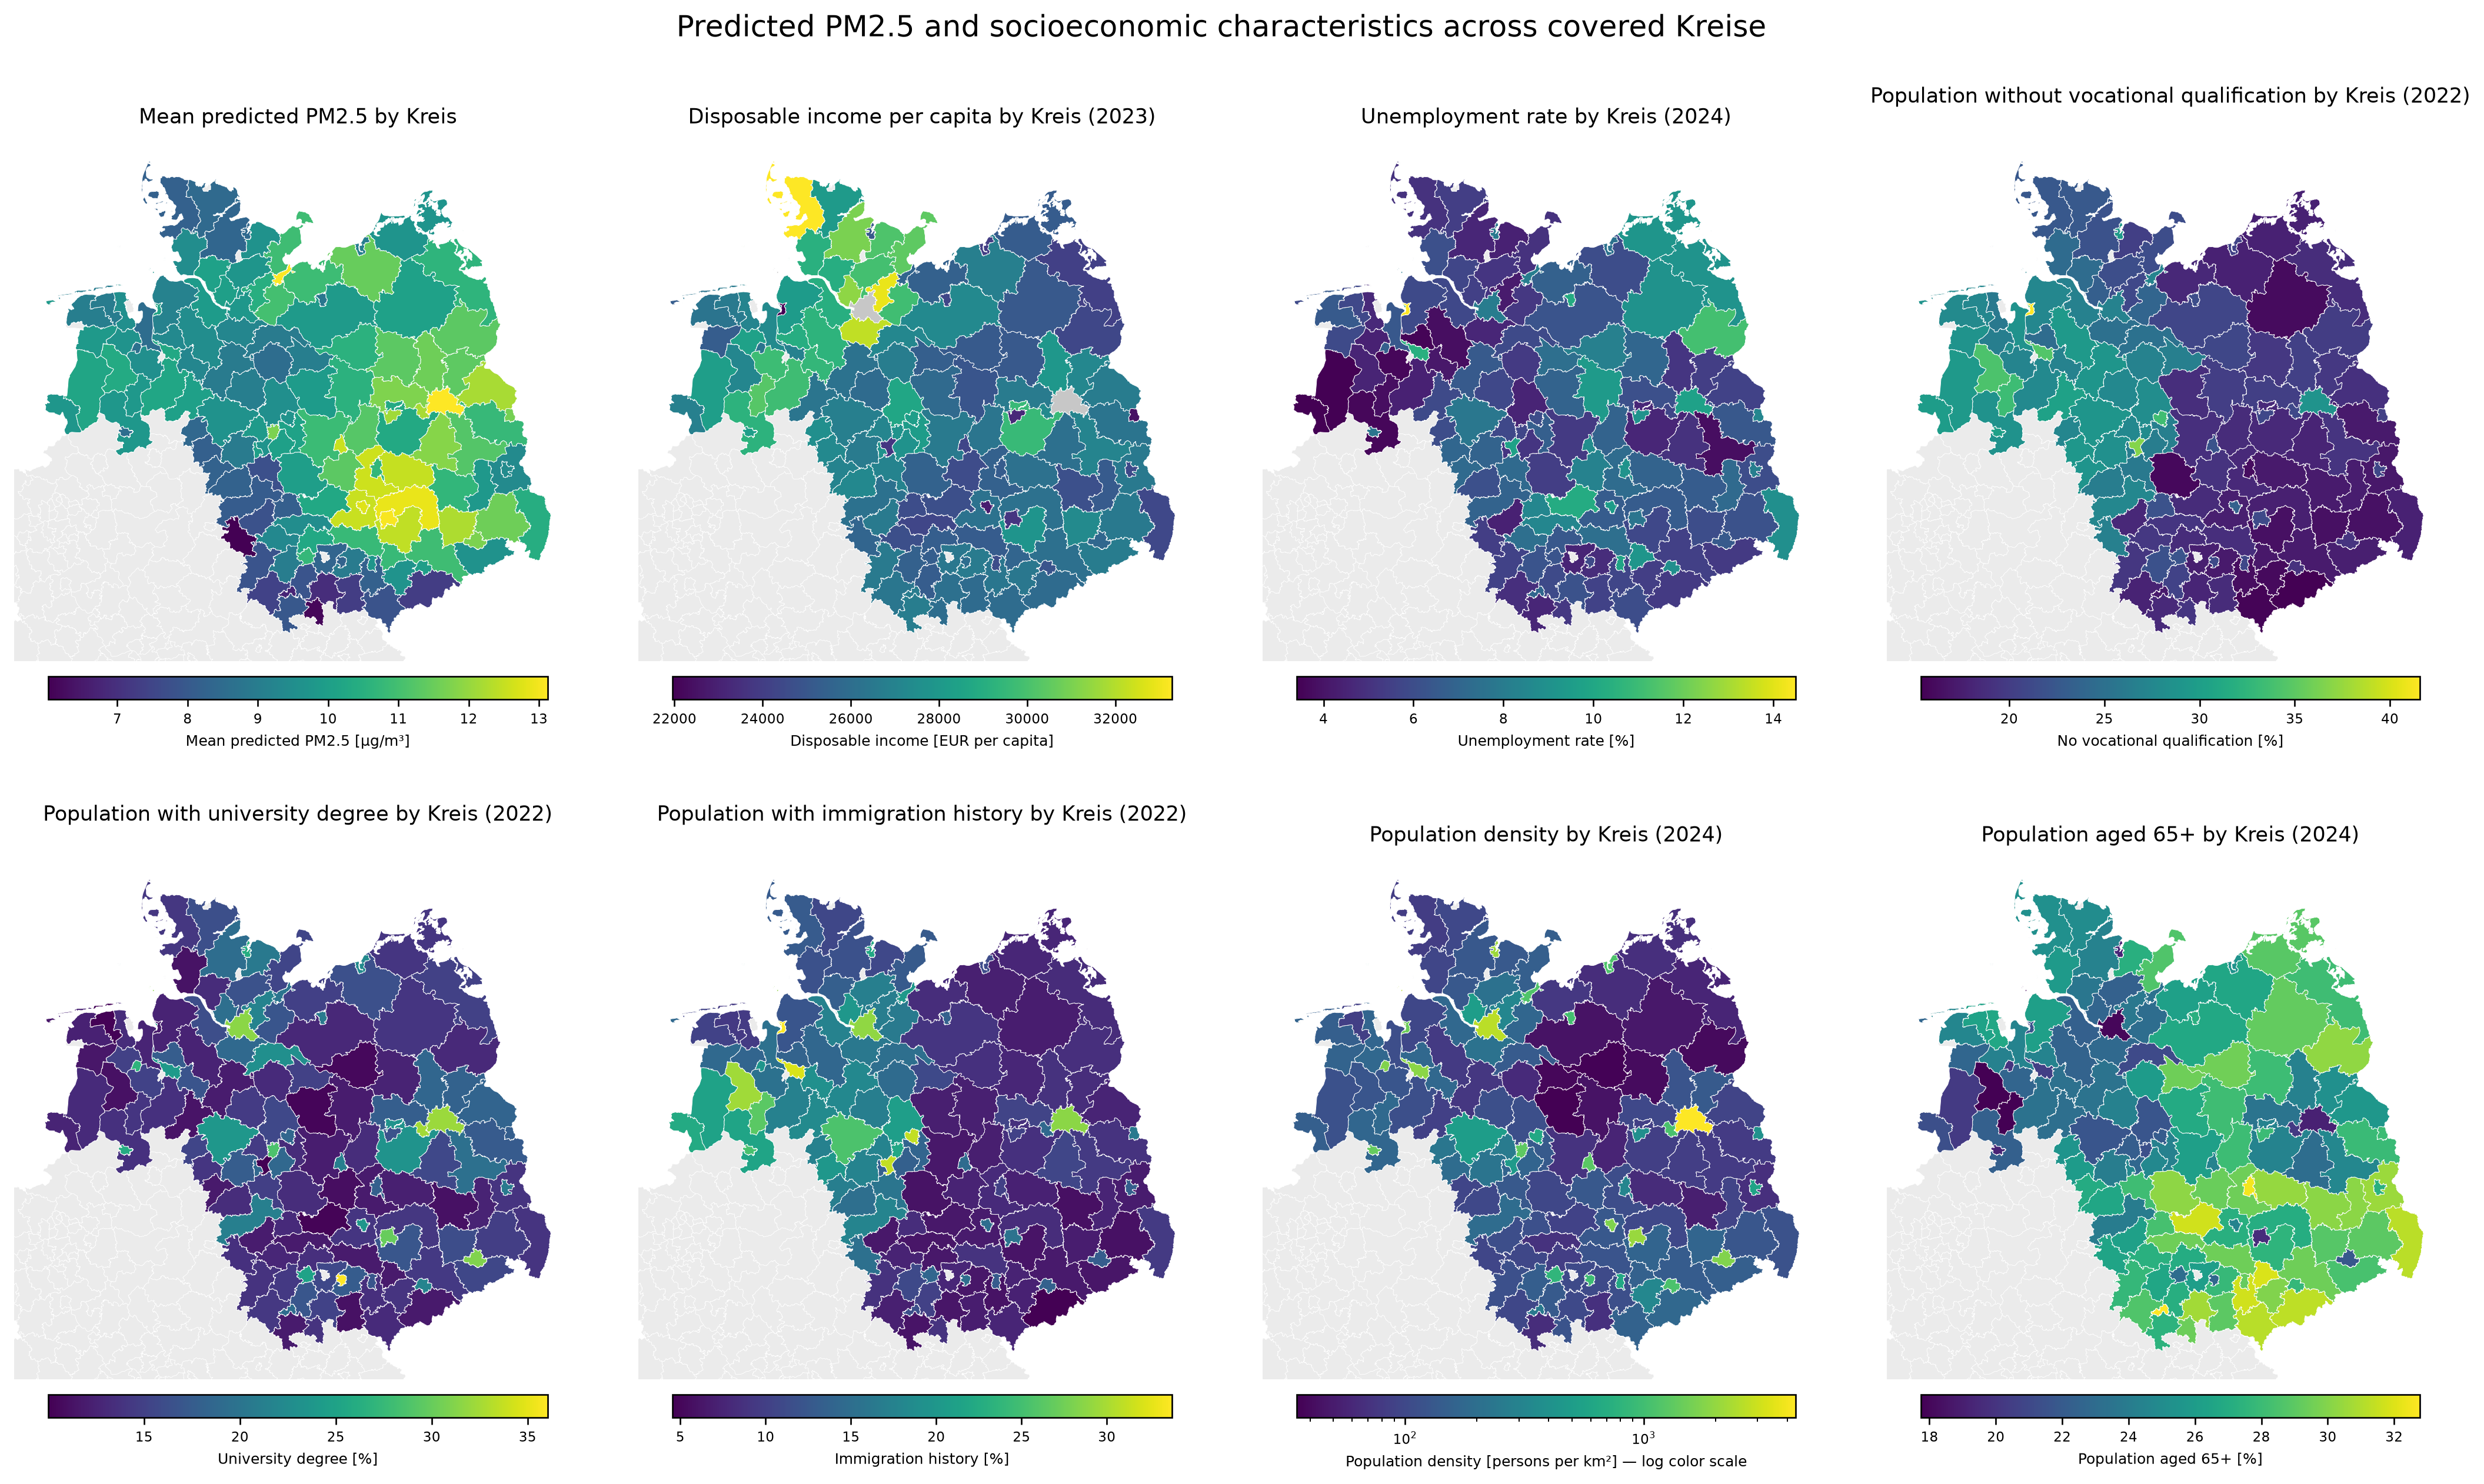
\includegraphics[width=\textwidth]
    {Figures/generated/socioeconomic_summary_maps.png}
    \caption{Mean predicted PM2.5 and selected socioeconomic and demographic characteristics across Kreise covered by the dense prediction grid.}
    \label{fig:socioeconomic_maps}
\end{figure}

\begin{figure}[ht]
    \centering
    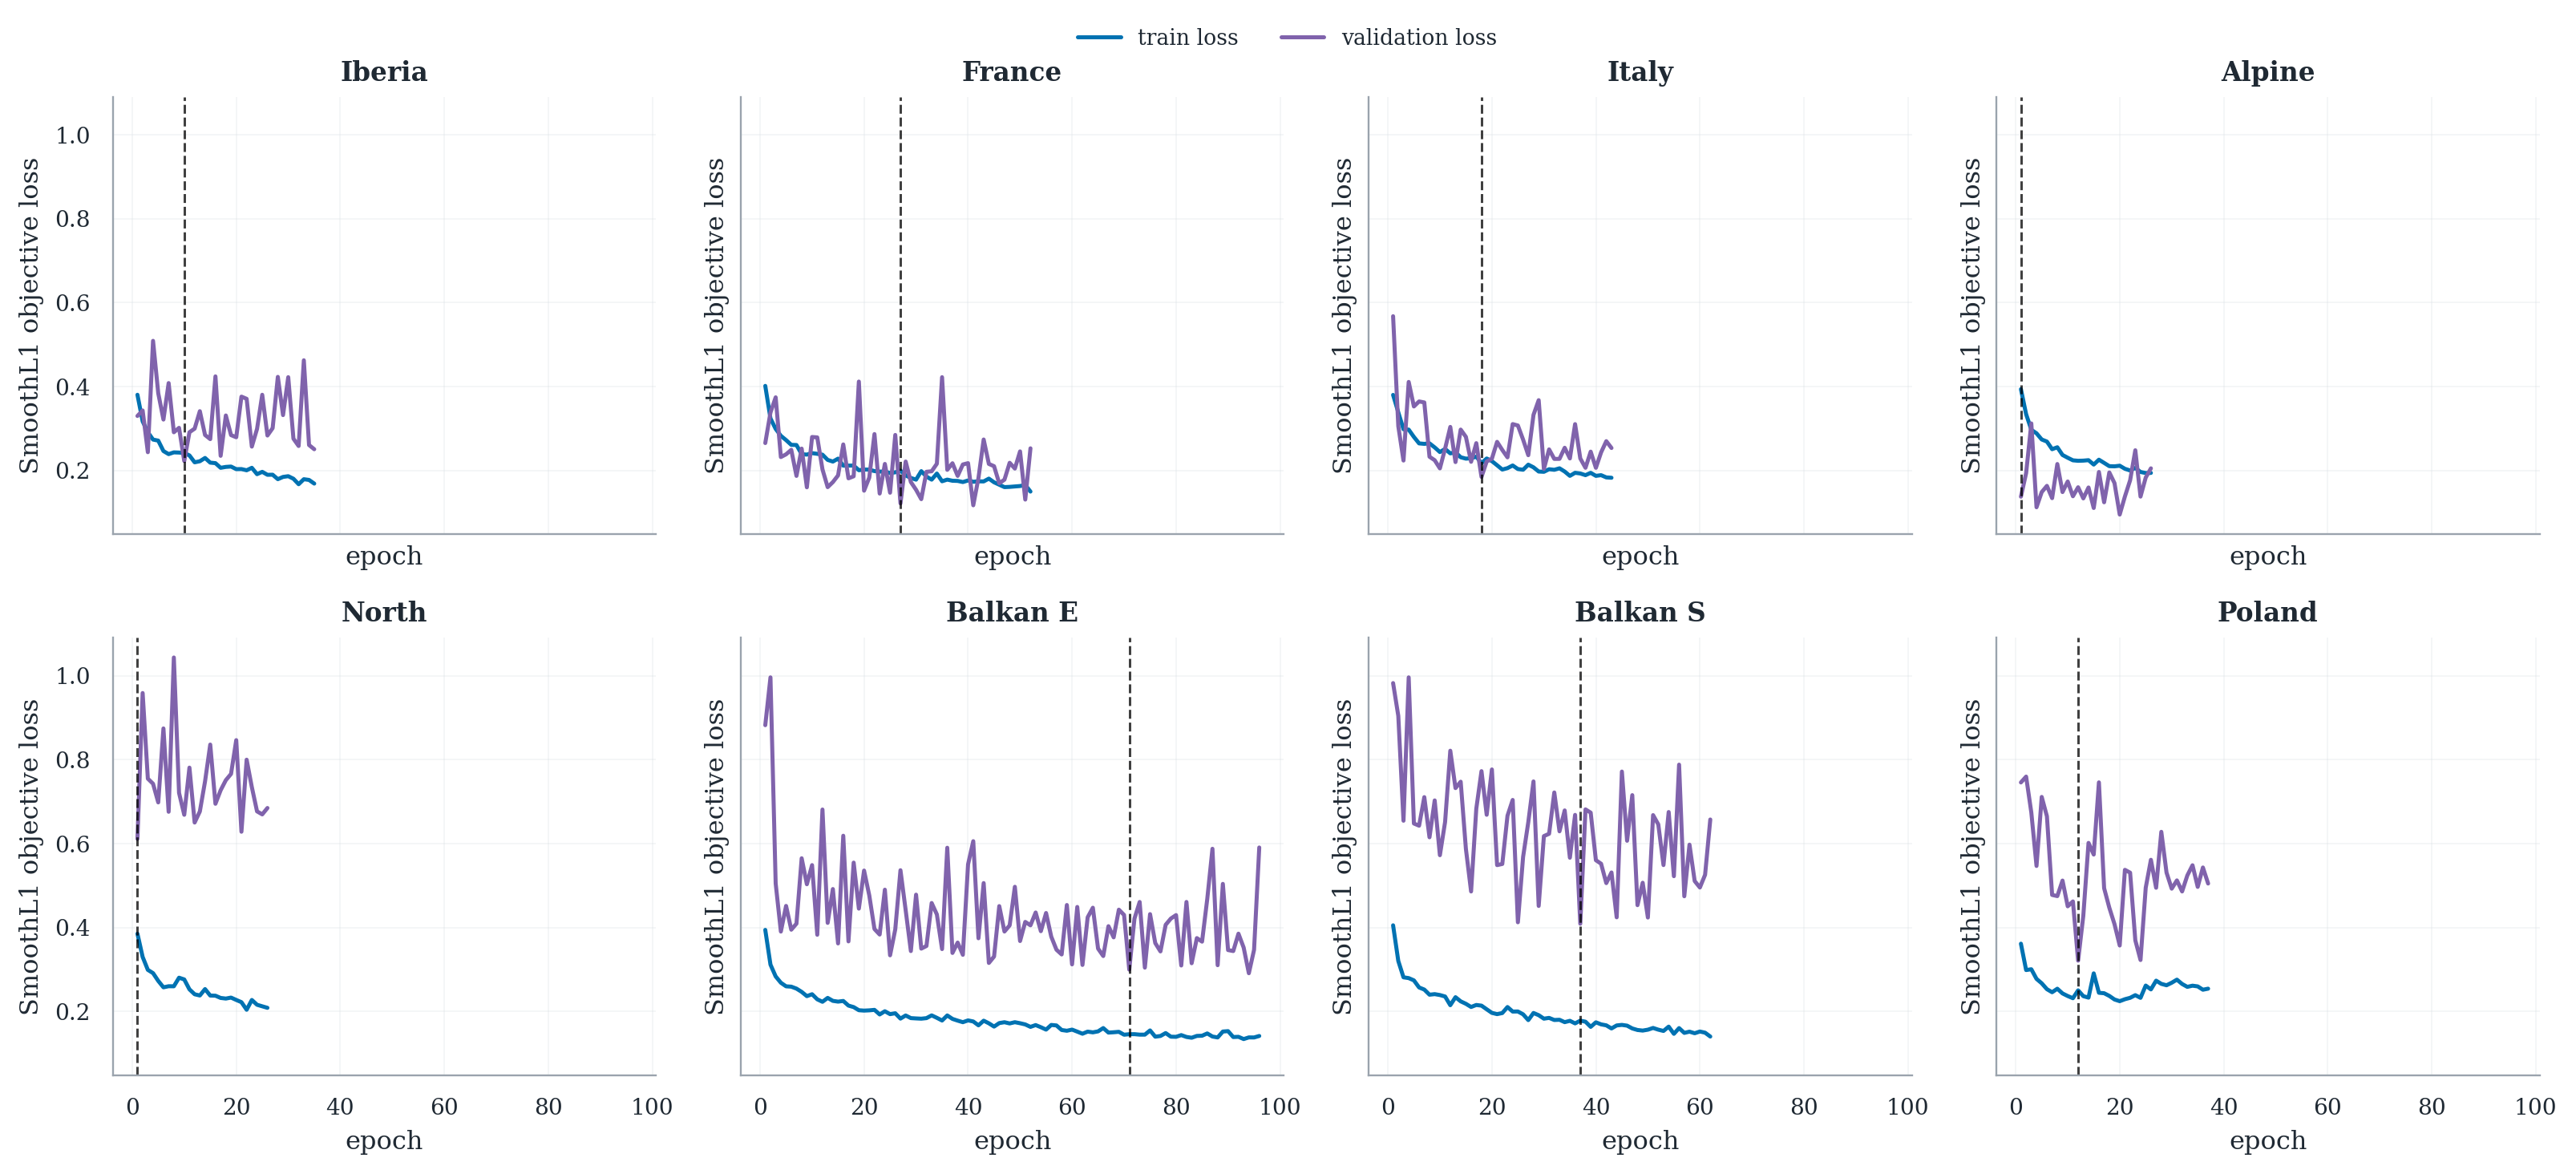
\includegraphics[width=\textwidth]{Figures/generated/learning_curves_cnn_deep_wide_objective_loss.png}
    \caption{Objective-loss learning curves for the scratch CNN (\texttt{cnn\_deep\_wide}) from the later reproducibility rerun, shown as a training diagnostic rather than as the original pre-TEST model-selection record.}
    \label{fig:learning_curves_cnn}
\end{figure}

\begin{figure}[ht]
    \centering
    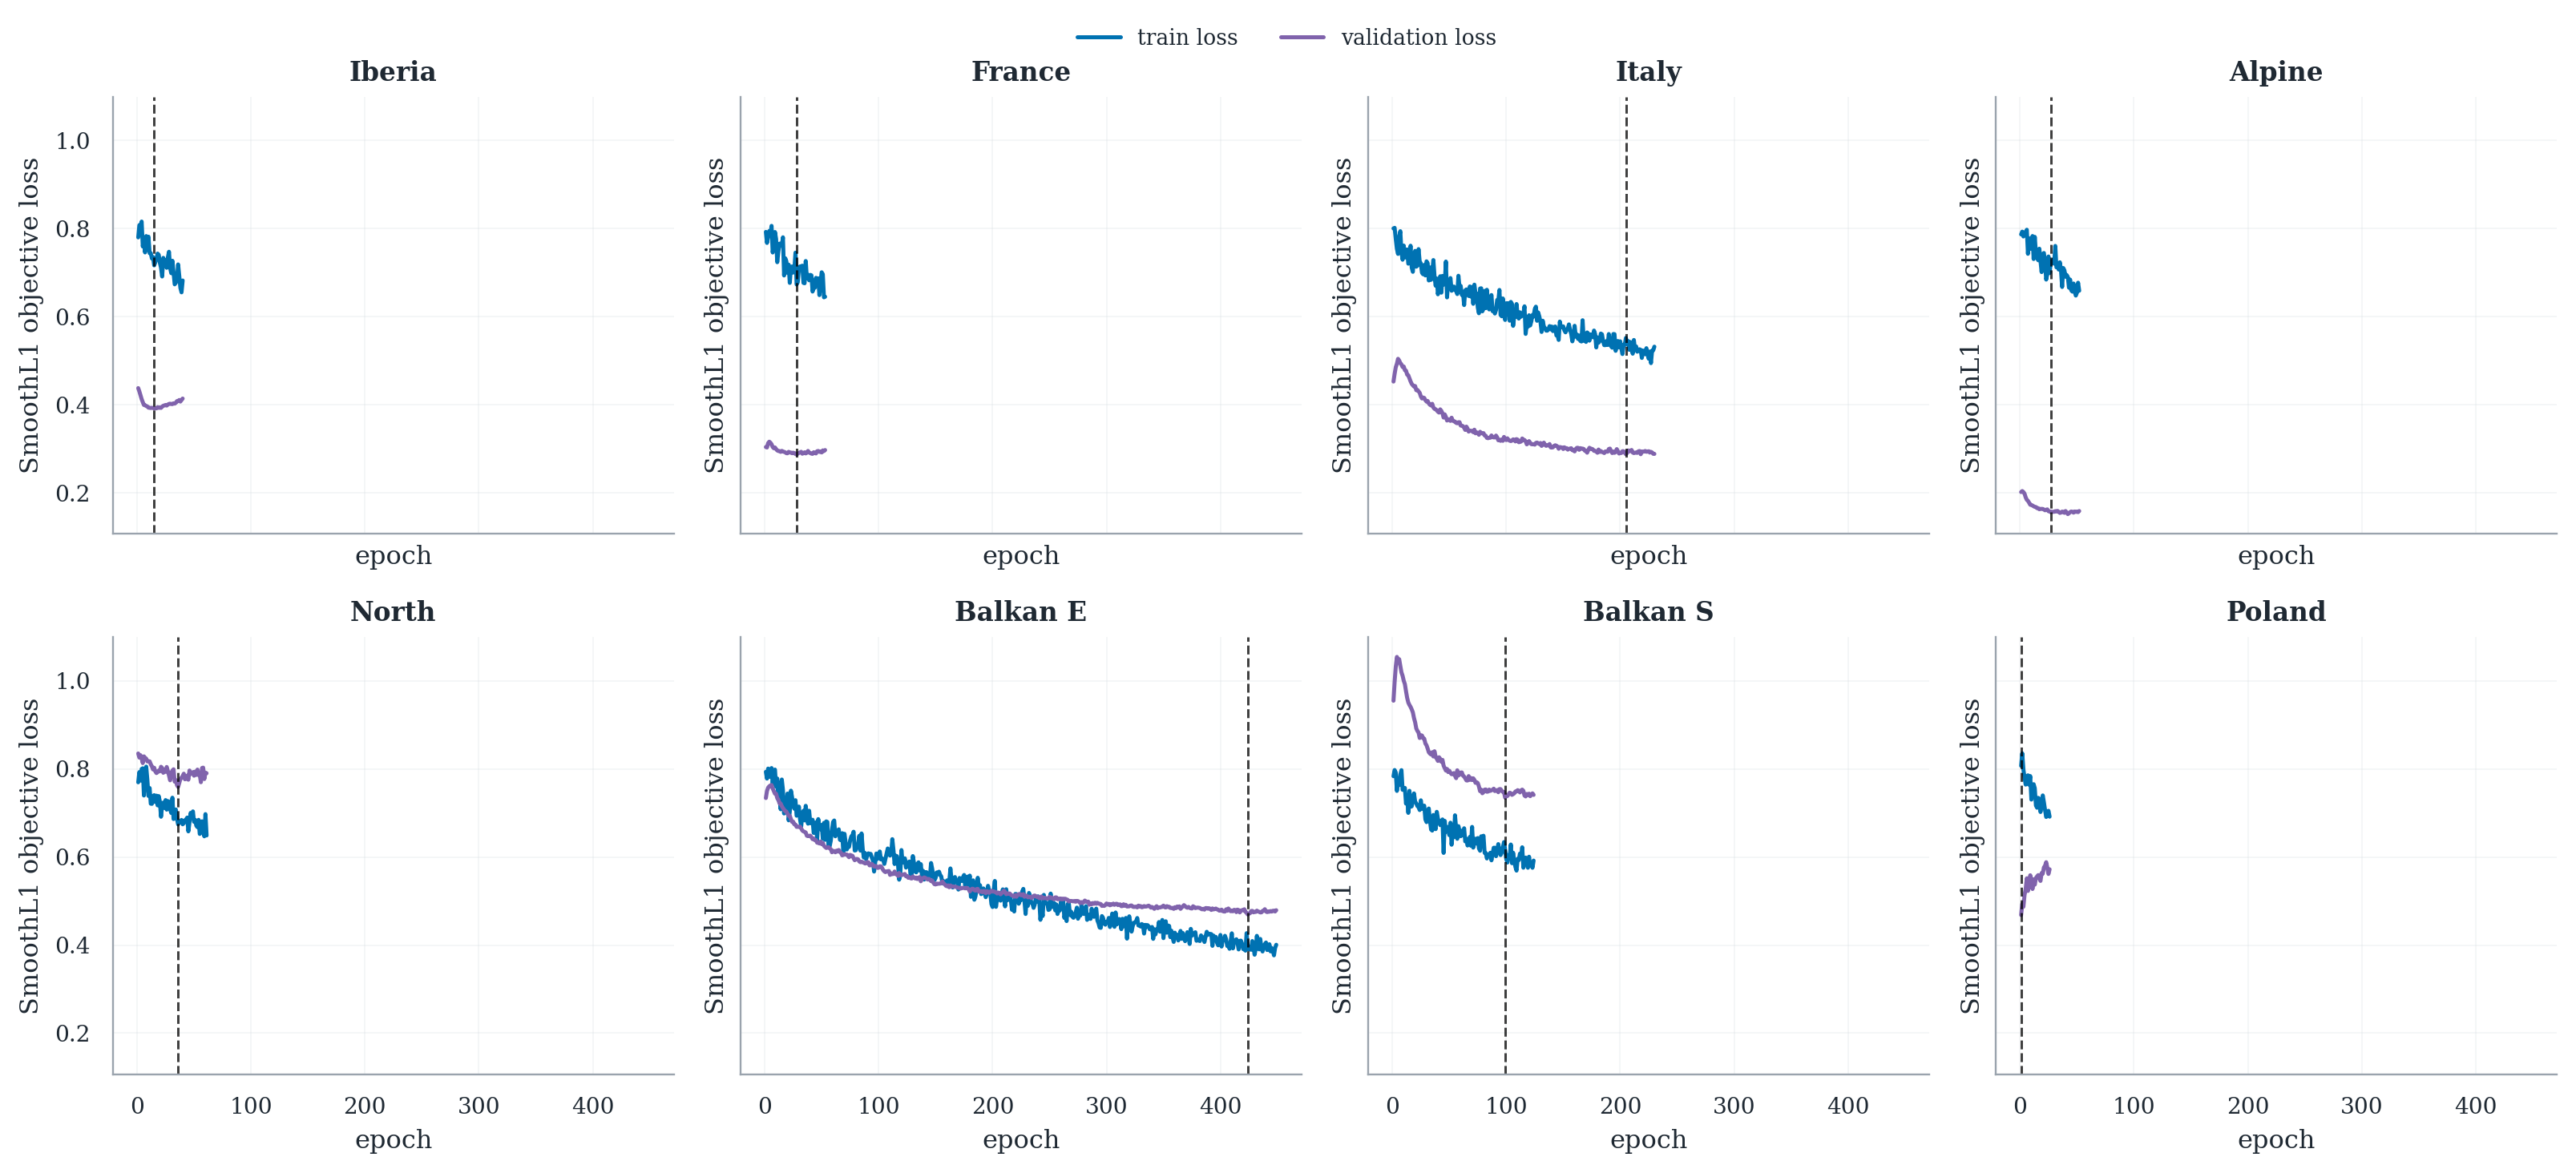
\includegraphics[width=\textwidth]{Figures/generated/learning_curves_resnet_frozen_objective_loss.png}
    \caption{Objective-loss learning curves for the frozen-backbone ResNet model from the later reproducibility rerun, shown as a training diagnostic rather than as the original pre-TEST model-selection record.}
    \label{fig:learning_curves_resnet}
\end{figure}

\begin{table}[ht]
\centering
\caption{Per-fold cross-validation results for the scratch CNN (\texttt{cnn\_deep\_wide}, PM2.5).}
\label{tab:cnn_deep_wide_folds}
\begin{tabular}{lccccc}
\hline
\textbf{Fold} & \textbf{Best epoch} & \textbf{RMSE} & \textbf{MAE} & \textbf{R}$^2$ & \textbf{Baseline RMSE} \\
\hline
fold1\_iberia    & 10 & 2.330 & 1.799 & 0.180  & 4.200 \\
fold2\_france    & 27 & 1.999 & 1.501 & -0.460 & 4.203 \\
fold3\_italy     & 18 & 3.508 & 2.749 & 0.329  & 5.051 \\
fold4\_alpine    & 1  & 1.946 & 1.502 & -0.187 & 3.377 \\
fold5\_north     & 1  & 3.419 & 3.002 & -1.579 & 5.271 \\
fold6\_balkan\_e & 71 & 6.168 & 4.290 & 0.002  & 8.297 \\
fold7\_balkan\_s & 37 & 6.681 & 4.838 & -0.020 & 9.400 \\
fold8\_poland    & 12 & 4.654 & 3.809 & -1.441 & 4.730 \\
\hline
Pooled out-of-fold ($n=1869$) & -- & 3.823 & 2.700 & 0.417 & -- \\
\hline
\end{tabular}
\end{table}

\begin{table}[ht]
\centering
\caption{Per-fold cross-validation results for the frozen-backbone ResNet-50 model (PM2.5).}
\label{tab:resnet_frozen_folds}
\begin{tabular}{lccccc}
\hline
\textbf{Fold} & \textbf{Best epoch} & \textbf{RMSE} & \textbf{MAE} & \textbf{R}$^2$ & \textbf{Baseline RMSE} \\
\hline
fold1\_iberia    & 15  & 3.085 & 2.628 & -0.437 & 4.200 \\
fold2\_france    & 28  & 3.037 & 2.788 & -2.369 & 4.203 \\
fold3\_italy     & 205 & 4.496 & 3.400 & -0.103 & 5.051 \\
fold4\_alpine    & 27  & 2.166 & 1.839 & -0.470 & 3.377 \\
fold5\_north     & 36  & 4.153 & 3.691 & -2.807 & 5.271 \\
fold6\_balkan\_e & 424 & 7.738 & 5.243 & -0.570 & 8.297 \\
fold7\_balkan\_s & 99  & 9.073 & 7.163 & -0.881 & 9.400 \\
fold8\_poland    & 1   & 5.551 & 4.834 & -2.472 & 4.730 \\
\hline
Pooled out-of-fold ($n=1869$) & -- & 4.895 & 3.663 & 0.045 & -- \\
\hline
\end{tabular}
\end{table}

\begin{table}[ht]
\centering
\caption{TEST-set performance by German federal state (\texttt{cnn\_deep\_wide}, PM2.5).}
\label{tab:test_by_state}
\begin{tabular}{lcccc}
\hline
\textbf{State} & \textbf{n} & \textbf{Bias} & \textbf{MAE} & \textbf{R}$^2$ \\
\hline
Berlin                  & 12 & 1.182 & 1.182 & 0.235 \\
Hamburg                 & 8  & 0.394 & 0.678 & -2.384 \\
Bremen                  & 4  & 0.370 & 0.625 & -26.02 \\
Sachsen                 & 19 & 2.052 & 2.146 & -1.790 \\
Niedersachsen           & 29 & 1.574 & 1.712 & -4.410 \\
Mecklenburg-Vorpommern  & 18 & 1.313 & 1.495 & -6.931 \\
Thueringen              & 21 & 1.738 & 2.054 & -4.744 \\
Brandenburg             & 25 & 1.853 & 1.853 & -7.683 \\
Schleswig-Holstein      & 10 & 2.381 & 2.579 & -8.270 \\
Sachsen-Anhalt          & 18 & 2.944 & 3.105 & -7.038 \\
\hline
\end{tabular}
\end{table}

\end{document}
